\documentclass[10pt, landscape, a4paper]{article}
\usepackage{geometry}[landscape]
\usepackage{multicol}
\usepackage{graphicx}
\usepackage{amsmath} 
\usepackage{amssymb}
\usepackage{ccicons}
\usepackage{hyperref}


\usepackage[boxruled, linesnumbered]{algorithm2e}

%% This declares a command \Comment
\SetKwComment{Comment}{/* }{ */}

\usepackage[dvipsnames]{xcolor}

% Set page margins
\geometry{top=.8cm, left=.8cm, right=.8cm, bottom=.8cm}

% Set paragraph indentation
\setlength{\parindent}{0pt}

% Set path for assets
\graphicspath{{assets/}}

\setlength{\columnsep}{20pt}
\raggedcolumns

% _____ CUSTOM COMMANDS __________________________________________
\newcommand{\E}[0]{\mathbb{E}}
\newcommand{\N}[0]{\mathbb{N}}
\newcommand{\R}[0]{\mathbb{R}}

\newcommand{\sgn}[0]{\text{sgn}}

\newcommand{\argmin}[1]{\underset{#1}{\text{argmin}}}
\newcommand{\argmax}[1]{\underset{#1}{\text{argmax}}}

\begin{document}
\begin{multicols*}{3}

% _____ CONTENT __________________________________________________

% main heading
\begin{center}
	\Large{\textbf{Computer Systems}} \\
    \small{by dcamenisch}
\end{center}

\section{Introduction}

This document is a summary of the 2022 edition of the lecture \textit{Computer Systems} at ETH Zurich. I do not guarantee correctness or completeness, nor is this document endorsed by the lecturers. If you spot any mistakes or find other improvements, feel free to open a pull request at \url{https://github.com/DannyCamenisch/systems-summary}. This work is published as CC BY-NC-SA.

\begin{center}
	\ccbyncsa
\end{center}

\begin{center}
	\Large{\textbf{Operating Systems}}
\end{center}

\section{Naming}

Naming is a fundamental concept, it allows resources to be bound at different times. Names are bound to objects, this is always relative to a context. One example of this would be path names, e.g. \textit{/usr/bin/emacs}. Name resolution can be seen as a function from context and name to some object. The resolved object can be a context in itself. This gives us a naming network.
\begin{center}
	\includegraphics[width=0.8\linewidth]{naming-network.png}
\end{center}

Both synonyms (two names bound to the same object) and homonyms (the same name bound to two different objects) can occur.
\section{The Kernel}

There are three main functions to an OS. Commonly they are referred to from a designer's view, but the user's view can be much more helpful to actually understand how it works.

\begin{center}
	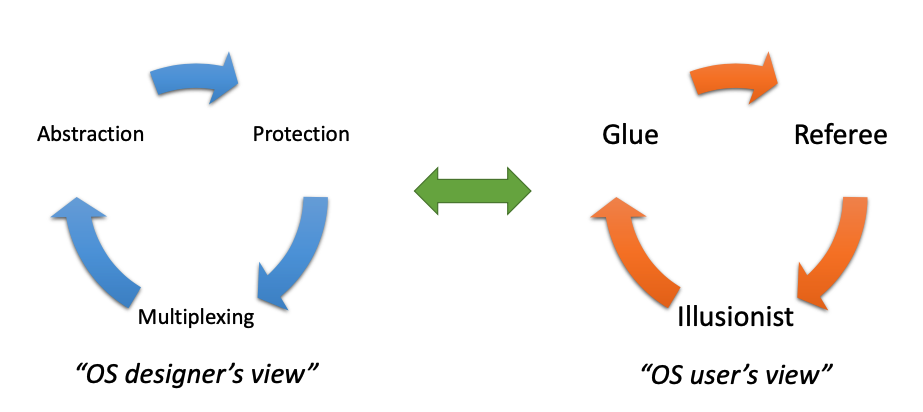
\includegraphics[width=\linewidth]{os-functions.png}
\end{center}


\subsection{Bootstrapping}

The term bootstrapping refers to pulling himself up from his own boots. In computer systems it is what we call the process of starting up a computer (booting). This boot process looks like this:

\begin{enumerate}
	\item CPU starts executing code at a fixed address (Boot ROM)
	\item Boot ROM code loads 2nd stage boot loader into RAM
	\item Boot loader loads kernel and optionally initials file system into RAM
	\item Jumps to kernel entry point
\end{enumerate}

The first few lines are always written in assembly, but generally we want to switch to C as soon as possible.


\subsection{Mode Switch}

One of our main goals is to protect the OS from applications that could harm it (intentionally or not). For this purpose we introduce two different modes:

\begin{itemize}
	\item \textbf{Kernel Mode} - execution with full privileges, read/write to any memory, access and I/O, etc. Code here must be carefully written
	\item \textbf{User Mode} - limited privileges, only those granted by the OS kernel
\end{itemize}

These two (or more) modes are already implemented in hardware. The main reason for a mode switch is when we encounter a processor exception (mode switch from user to kernel mode). If this is the case, we want the following to happen:

\begin{enumerate}
	\item Finish executing current instruction
	\item Switch mode from user to kernel
	\item Look up exception cause in exception vector table
	\item Jump to this address
\end{enumerate}

Further we may also want to save the registers and switch page tables. When switching between the modes we also have to change our address space, but we might want to access some informations from the user mode address space. One way of doing this is to use a so called \textbf{trampoline}, which is a part of the address space that gets mapped to the same location in user and kernel mode.

\begin{center}
	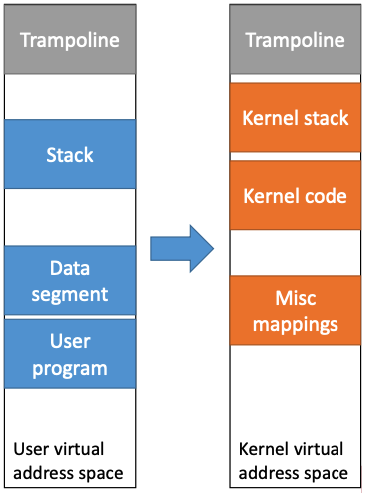
\includegraphics[width=0.4\linewidth]{trampoline.png}
\end{center}

Mode switches can also occur the other way around (from kernel mode to user mode). The main reasons for this are:

\begin{itemize}
	\item New process / thread start
	\item Return from exception
	\item Process / thread context switch
	\item User-level upcall (UNIX signal)
\end{itemize}

This leads us to the following perspective:

\begin{center}
	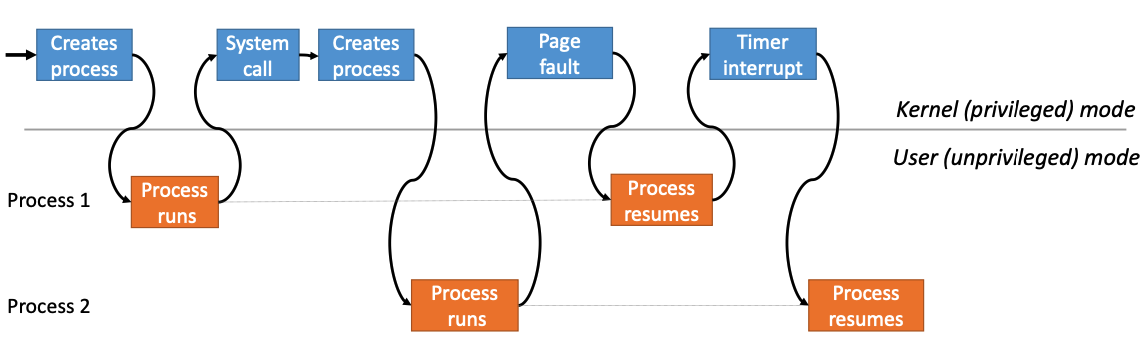
\includegraphics[width=\linewidth]{mode-switch.png}
\end{center}

The mode switch is fundamental to modern computers:

\begin{itemize}
	\item It enables virtualization of the processor
	\item It creates the illusion of multiple computers
	\item It referees access to the CPU
\end{itemize}


\subsection{General Model of OS Structure}

\begin{center}
	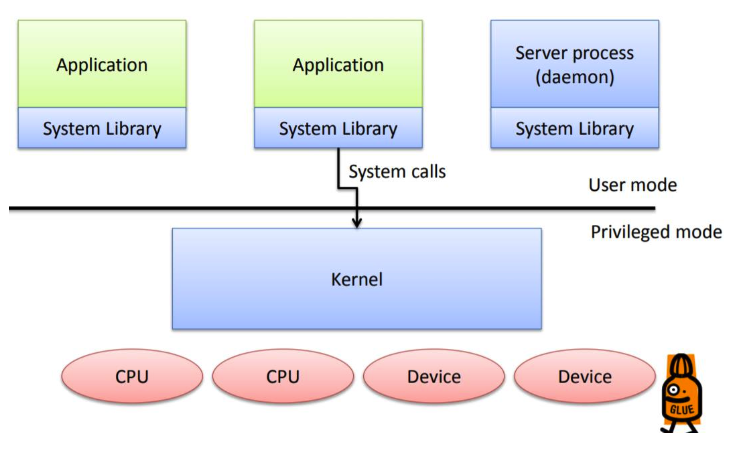
\includegraphics[width=0.9\linewidth]{os-structure.png}
\end{center}

\begin{itemize}
	\item \textbf{Kernel}: The kernel consists of software run in privileged mode. There might be more than one kernel in an OS. It can handle system calls, h/w interrupts etc.
	\item \textbf{System Libraries}: They are part of any application run on the machine and should provide an interface for the kernel.
	\item \textbf{Daemon}: This is a process running as part of the OS. It’s not run in privileged mode and may use system libraries. An example might be a file system.
\end{itemize}

We can differentiate between monolithic kernels and microkernels, depending on the amount of code in kernel mode.


\subsection{System Calls}

System calls are the only way for user mode programs to enter kernel mode. System calls are a type of exception, but they try to look a lot more like a procedure call. Therefore the kernel system call handler has to first locate arguments, copy these arguments into kernel memory, validate these arguments and then copy the results back into user memory after execution. An example of such a system call would be \textit{write()}. 


\subsection{Hardware Timers}

What happens if a user mode program does not cause any exception and does not give control back to the kernel? Hardware timers are a solution for this problem, the hardware device periodically interrupts the processor and returns control to the kernel handler, which sets the time of the next interrupt.

\section{Processes}

When you run a program, the OS creates a process to execute the program in. A process is an illusion created by the OS, it creates an execution environment for a program. This environment gives the program limited rights (access, name spaces, threads, etc.) and therefore it is both a security and a resource principal.


\subsection{Creating a Process}

There are two main approaches to creating new processes:

\begin{itemize}
	\item \textbf{Spawn} - constructs a running process from scratch
	\item \textbf{Fork / Exec} - creates a copy of the calling process or replaces the current program with another in the same process
\end{itemize}

\textbf{Spawn}

\begin{itemize}
	\item Create and initialize the process control block (PCB) in the kernel
	\item Create and initialize a new address space
	\item Load the program into the address space
	\item Copy arguments into memory in the address space
	\item Initialize the hardware context to start execution at "start"
	\item Inform the scheduler that the new process is ready to run
\end{itemize}

Spawn is very complex, we have to specify everything about the new environment. If we omit a key argument a new process might have insufficient rights or resources or it might fail to function due to a security fault. \medskip

\textbf{Fork}

Fork on the other hand is less complex. The child process is almost an exact copy of the parent, with a different PID. We know which process we are in from the return value of the \textit{fork()} call ($0$ for child, $>0$ for parent, $<0$ for error). The complete UNIX process management API also includes:

\begin{itemize}
	\item \textit{exec()} - system call to change the program being run by the current process
	\item \textit{wait()} - system call to wait for a process to finish
	\item \textit{signal()} - system call to send a notification to another process
\end{itemize}

In contrast to \textit{spawn()}, here the child revokes rights and access explicitly before \textit{exec()}, further we can use the full kernel API to customize the execution environment.


\subsection{The Process Control Block}

The PCB is the main kernel data structure used to represent a process. It has to hold or refer to the page table, trap frame, kernel stack, open files, program name, scheduling state, PID, etc.


\subsection{Process Context Switching}

Context switching is the process of switching between different processes running in user mode or kernel mode. It is one of the key elements of the illusion that multiple programs can run in parallel. \columnbreak

There are two main reasons for the kernel to switch processes: either when a process has run for too long and gets interrupted by a hardware timer or when a process blocks. The second case happens when a system call can not complete immediately. The process then often calls \textit{sleep()} and other processes can be executed.
\begin{center}
	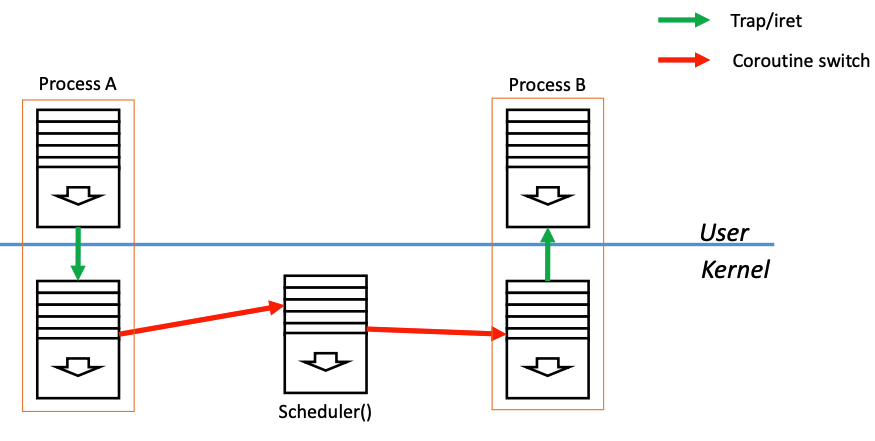
\includegraphics[width=\linewidth]{context-switching.png}
\end{center}


\subsection{Process Hierarchy}

By forking and spawning new processes we create sort of a hierarchy. If a child process dies, but the parent does not call \textit{wait()}, the child process becomes a zombie - it is dead, but still around since nobody asked for the return code. If a parent dies, but the child does not, the child becomes an orphan and gets reparented to the first process (PID \#1, \textit{init}).
\begin{center}
	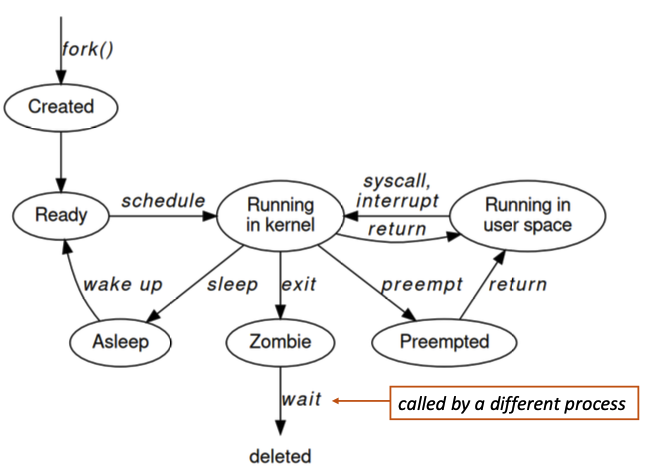
\includegraphics[width=\linewidth]{process-life-cycle.png}
\end{center}

The \textit{init} process is basically an infinite loop calling \textit{wait}(NULL), it gets rid of any zombies.


\subsection{Threads}

Threads are used as an abstraction for concurrency. They allow the usage of parallel hardware, e.g. multiple cores. A thread basically consist of a stack and some register values.\medskip

There is a distinction between \textbf{user threads} and \textbf{kernel threads}. The former are implemented entirely in user’s process. If a user thread is about to block (e.g. when executing a system call), the thread library usually interrupts this call and does something non blocking instead while the system call is served. Kernel threads are implemented by the OS kernel directly. They thus appear as different virtual processors to the user process. In this model, a set of threads share a virtual address space together. Each thread is now scheduled by the kernel itself, which keeps track of threads are part of which process. However, this makes the kernel more complicated.

\section{Inter-Process Communication}

It is often the case, that we want different processes to work together, e.g. DB and web-scraper. For this we need ways to exchange information between processes, we call this inter-process communication or IPC.\medskip

One of the most basic ways to exchange information is system calls. We save our data on the stack or in a register and execute the system call, the kernel then switches execution to the other process with the information about the data that should be exchanged. This is a really flawed approach some reasons are that context switches are expensive and it is unsafe to introduce new system calls for each task.

\subsection{Shared Memory}

We introduce shared memory that can only be accessed by the processes that communicate with each other. This requires us to define a common interface between the processes. The main building blocks for this are:
\begin{itemize}
	\item Shared area: registers, memory - define the layout of the memory
	\item Indicating status: shared variables, signals
	\item Updating status: changing variables
	\item Consistency: use synchronization primitives
\end{itemize}

When checking the state of a shared variable polling can be very inefficient. As an alternative we can use a signal handler. When the first process calls the signal handler, the kernel notifies the second process of the update. When the kernel issues such a system call to a process, we call it an \textbf{upcall}. To guarantee consistency, we use synchronization primitives that are already known from previous lectures (spin locks with CAS, TAS, etc.). \medskip

A more modern approach is to use transactional memory, hereby we work with transactions that can fail on race condition.

\section{Scheduling}

First we introduce some terminology, notice how the wait time is defined as the combination of hold time and execution time.
\begin{center}
	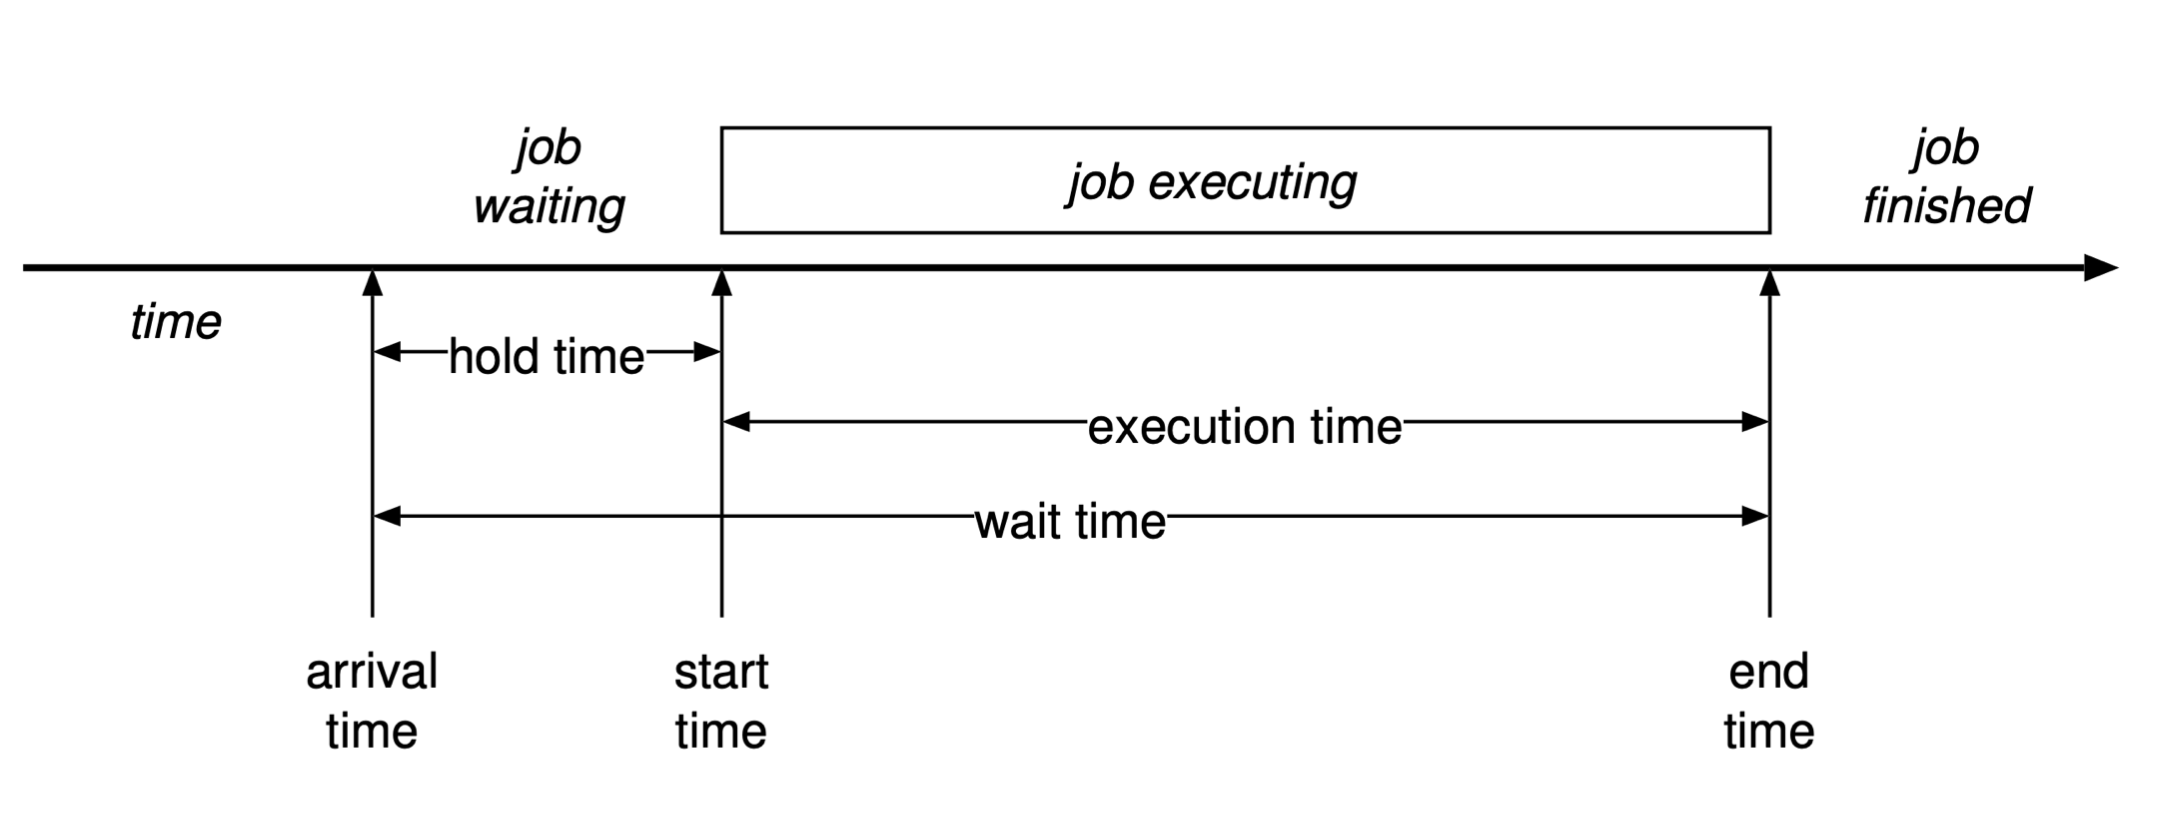
\includegraphics[width=\linewidth]{scheduling.png}
\end{center}

The important metrics for scheduling are throughput (rate of completing jobs) and overhead (time spent without a job executing).

In the following part we will look at various scheduling algorithms, starting from a very simple approach.

\subsection{Non-Preemptive Batch Oriented}

There are two basic algorithms:
\begin{itemize}
	\item First Come First Served
	\item Shortest Job First
\end{itemize}

Both are algorithms are very simple to implement but their applications are limited.

\subsection{Preemptive Batch Oriented}

We introduce preemption, meaning that we interrupt the execution after some finite time interval. After such an interrupt we decide which program to run next. \smallskip

\textbf{Modified SJF:} Go through the sorted list of jobs and execute each until interrupted. Note that the length of a job does not get recomputed after an execution. \smallskip

\subsection{Interactive Scheduling}

When running interactive workload, we can encounter events that block the execution (I/O, page-faults, etc.). During this time we would like to run another program instead of wasting execution time. \smallskip

\textbf{Round Robin Scheduling:} Let $R$ be a queue and $q$ be the scheduling quantum:
\begin{enumerate}
	\item Set an interval timer for an interrupt $q$ seconds in the future
	\item Dispatch the job at the head of $R$
	\item If blocking happens or the timer runs out, return to the scheduler
	\item Push the previously running job to the tail of $R$
\end{enumerate}

\textbf{Priority Based Scheduling:} We assign a priority to each task and dispatch the highest priority task first, if we have ties we use RR to break them. To avoid starvation we might want to use dynamic priorities (increased priority depending on wait time). An even more complex approach is to introduce multi-level queues, meaning that we have a fixed number of queues that assign priorities within each queue. Then we use RR scheduling between the queues to execute tasks. \medskip

Priority scheduling runs into problems when a high priority process has to wait for a lock from a low priority process (Priority Inversion). To fix this, we can either introduce inheritance - the holder of the lock acquires the priority of the highest waiting process - or ceiling - the holder of the lock runs at the highest priority.

\subsection{Linux o(1) Scheduler}

Linux uses 140 multilevel feedback queues, each with a different priority. Multilevel feedback queues penalize CPU bound tasks and prioritize I/O operations, as I/O tasks will eventually block.

The priority range 0-99 is used for high priority, static tasks and it uses FCFS or RR scheduling. The range 100-139 is for user tasks and uses RR together with priority ageing for I/O tasks.


\section{Input / Output}

Every OS has an I/O subsystem, which handles all interaction between the machine and the outside world. The I/O subsystem abstracts individual hardware devices to present a more or less uniform interface, provides a way to name I/O devices, schedules I/O operations and integrates them with the rest of the system, and contains the low-level code to interface with individual hardware devices. \medskip

To an OS programmer, a \textbf{device} is a piece of hardware visible from software. It typically occupies some location on a bus or I/O interconnect, and exposes a set of hardware registers which are either memory mapped or in I/O space. A device is also usually a source of interrupts, and may initiate Direct Memory Access (DMA) transfers. \medskip

The \textbf{device driver} for a particular device is the software in the OS which understands the specific register and descriptor formats, interrupt models, and internal state machines of a given device and abstracts this to the rest of the OS.

\subsection{Data Transfer}

\textbf {Programmed I/O} consists of causing input/output to occur by reading/writing data values to hardware registers. This is the simples form of communication. It is fully synchronous, so the CPU always has to be involved. Further it is polled, the device has no way to signal that new data is ready. \medskip

\textbf{Interrupts} can be used to signal the availability of new data and solve the polling problem. But the problem of CPU involvement still persists.
\begin{center}
	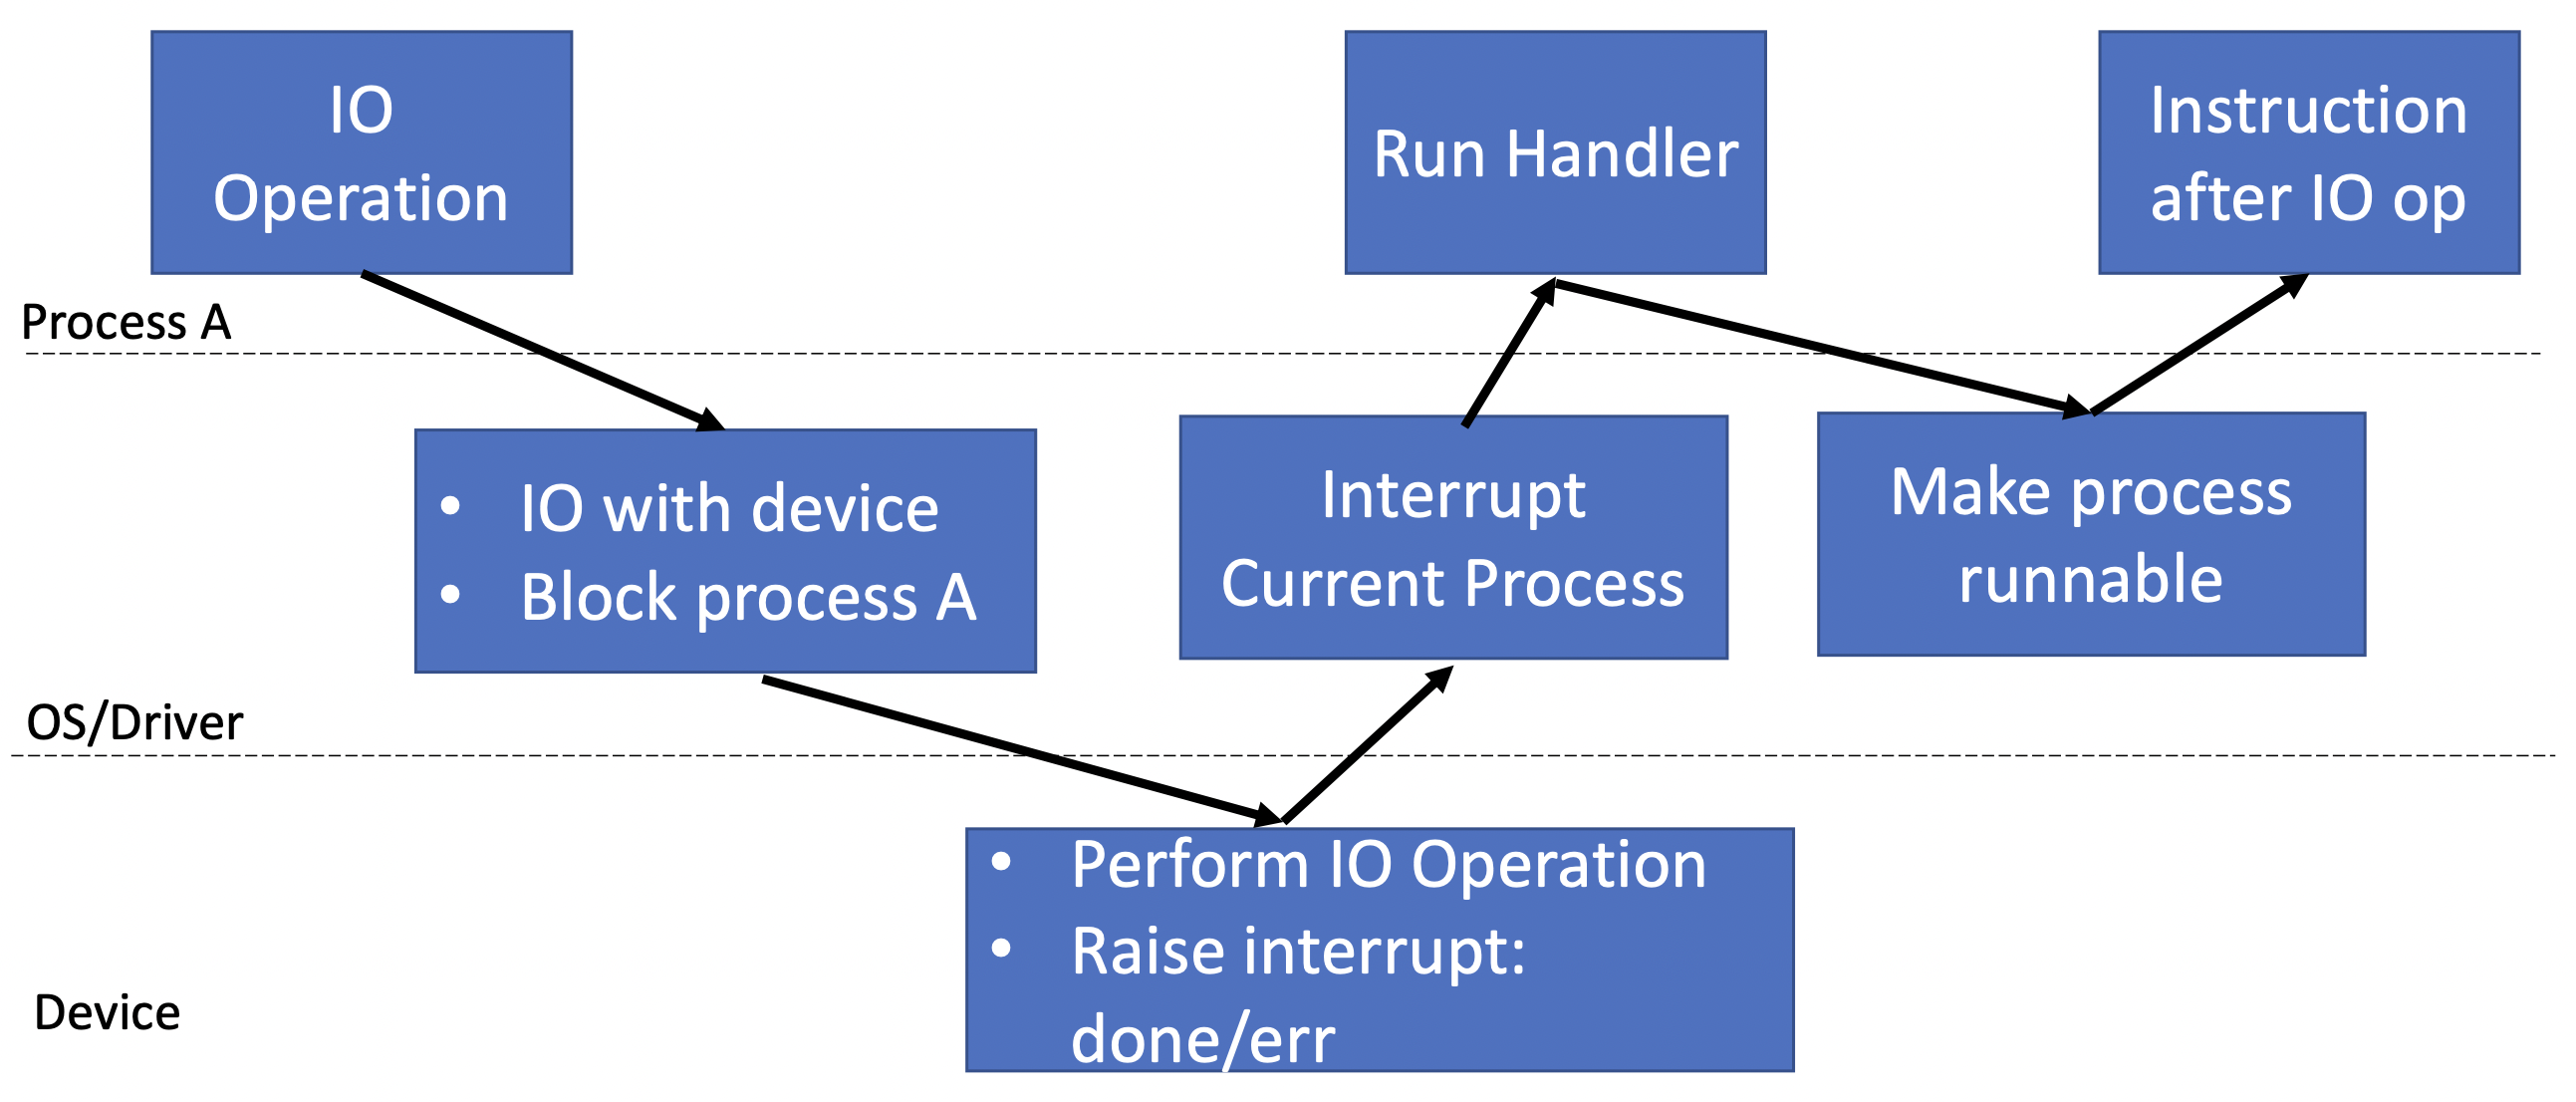
\includegraphics[width=\linewidth]{data_transfer_interrupt.png}
\end{center}

\textbf{Direct Memory Access} or DMA, a device can be given a pointer to buffers in main memory and transfer data to and from those buffers without further involvement from the CPU. A single interrupt is used to signal the end of data transfer. DMA is, for the most part, physical (not virtual) access to memory. Further DMA transfers to and from main memory may or may not be coherent with processor caches.

\subsection{Asynchrony}

Device drivers have to deal with the fundamentally asynchronous nature of I/O: the system must respond to unexpected I/O events, or to events which it knows are going to happen, but not when. \medskip

The \textbf{First-level Interrupt Service Routine} (FLISR) is the code that executes immediately as a result of the interrupt. It runs regardless of what else is happening in the kernel. As a result, it can't change much since the normal kernel invariants might not hold. \medskip

Since I/O is for the most part interrupt-driven, but data is transferred to and from processes which perform explicit operations to send and receive it. Consequently, data must be buffered between the process and the interrupt handler, and the two must somehow rendezvous to exchange data. There are three canonical solutions to this problem:

A \textbf{deferred procedure call}, is a program closure created by the 1st-level interrupt handler. It is run later by any convenient process, typically just before the kernel is exited. \medskip

A \textbf{driver thread}, sometimes called an interrupt handler thread, serves as an intermediary between ISR and processes. The thread starts blocked waiting for a signal either from the user process or the ISR. When an interrupt occurs or a user process issues a request, the thread is unblocked (this operation can be done inside an ISR) and it performs whatever I/O processing is necessary before going back to sleep. Driver threads are heavyweight: even if they only run in the kernel, the still require a stack and a context switch to and from them to perform any I/O requests. \medskip

The third alternative, is to have the FLISR convert the interrupt into a message to be sent to the driver process. This is conceptually similar to a DPC, but is even simpler: it simply directs the process to look at the device. However, it does require the FLISR to synthesize an IPC message, which might be expensive. In non-preemptive kernels which only process exceptions serially, however, this is not a problem, since the kernel does not need locks. \medskip

\textbf{Bottom-half handler} - the part of a device driver code which executes either in the interrupt context or as a result of the interrupt. \medskip

\textbf{Top-half handler} - the part of a device driver which is called "from above", i.e. from user or OS processes.

\subsection{Device Models}

The device model of an OS is the set of key abstractions that define how devices are represented to the rest of the system by their individual drivers. It includes the basic API to a device driver, but goes beyond this: it encompasses how devices are named throughout the system, and how their interconnections are represented as well. \medskip

\textbf{UNIX device model:}
\begin{itemize}
	\item Character Devices - used for unstructured I/O and present a byte-stream interface with no block boundaries.
	\item Block Devices - used for structured I/O and deal with blocks of data at a time.
	\item Network Devices - correspond to a network interface adapter. It is accessed through a rather different API.
	\item Pseudo Devices - a software service provided by the OS kernel which it is convenient to abstract as a device, even though it does not correspond a physical piece of hardware.
\end{itemize}

\subsection{Protection}

Another function of the I/O subsystem is to perform protection. Ensuring that only authorized processes can access devices or services offered by the device driver and that a device can't be configured to do something harmful. Unix controls access to the drivers themselves by representing them as files, and thereby leveraging the protection model of the file system. DMA-capable devices are in principle capable of writing to physical memory anywhere in the system, and so it is important to check any addresses passed to them by the device driver. Even if you trust the driver, it has to make sure that it’s not going to ask the device to DMA somewhere it shouldn’t. One approach is to put a memory management unit (MMU) on the path between the device and main memory, in addition to each core having one.

\section{Virtual Memory}

From previous courses we know MMUs, TLBs and basic paged virtual memory operations. The uses for address translation include: Process Isolation, Shared Code Segments, Dynamic Memory Allocation and many more.


\subsection{Segments}

Before paging, there were segments. Before segments there where base and limit registers. These contained two addresses $B$ and $L$. A CPU access to an address $a$ is permitted iff $B \leq a < L$. Relocation registers are an enhanced form of base register. All CPU accesses are relocated by adding the offset: a CPU access to an address $a$ is translated to $B + a$. This allows each program to be compiled to run at the same address (e.g. 0x0000). \medskip
\begin{center}
	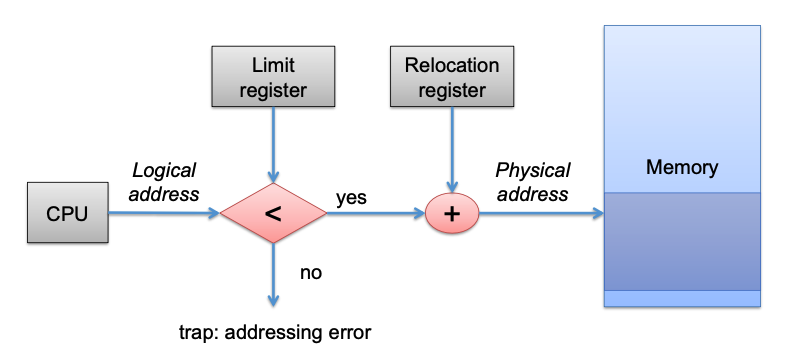
\includegraphics[width=\linewidth]{base-relocation-register.png}
\end{center}

A segment is a triple $(I, B_I, L_I)$ of values specifying a contiguous region of memory address space with base $B_I$, limit $L_I$, and an associated segment identifier $I$ which names the segment. Memory in a segmented system uses a form of logical addressing: each address is a pair $(I, O)$ of segment identifier and offset. A Segment Table is an in-memory array of base and limit values $(B_I, L_I)$ indexed by segment identifier, and possibly with additional protection information.
\begin{center}
	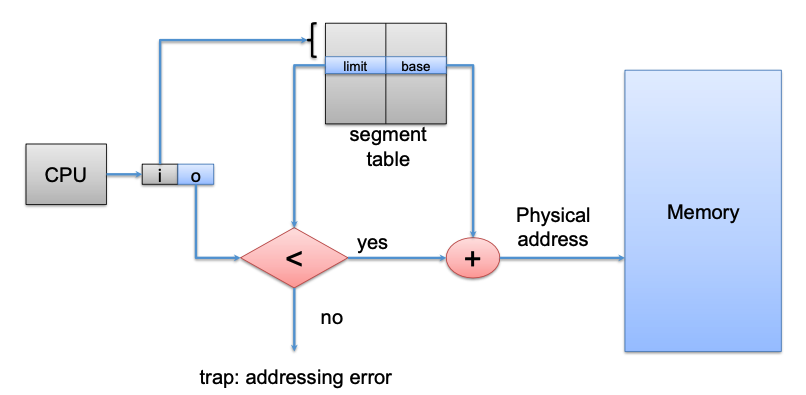
\includegraphics[width=\linewidth]{segment.png}
\end{center}

This enables sharing code/data segments between processes, further it adds protection and allows transparently growing stack/heap as needed. The principal downside of segmentation is that segments are still contiguous in physical memory, which leads to external fragmentation.


\subsection{Paging}

This is a short recap of paging. Virtual memory is divided into (virtual) pages of the same size having a VPN, physical memory gets divided into frames / physical pages having a PFN / PPN. Then a page table gets used to map VPNs to PFNs. This is implemented in hardware as the MMU. To speed up translation the TLB is used. Getting data from memory can work as follows (in this case we have a TLB miss):
\begin{center}
	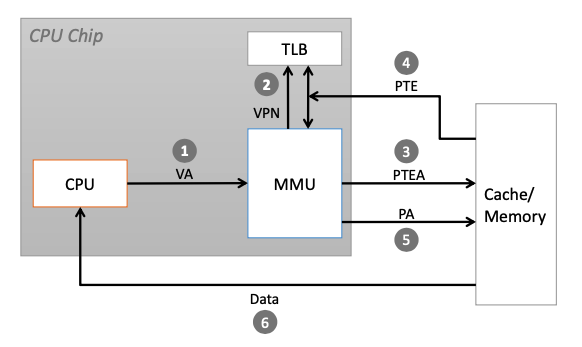
\includegraphics[width=\linewidth]{tlb-miss.png}
\end{center}

We have also seen how multi-level page tables work. Multi-level translation allows us to allocate only page table entries that are in use and makes memory allocation simpler.
\begin{center}
	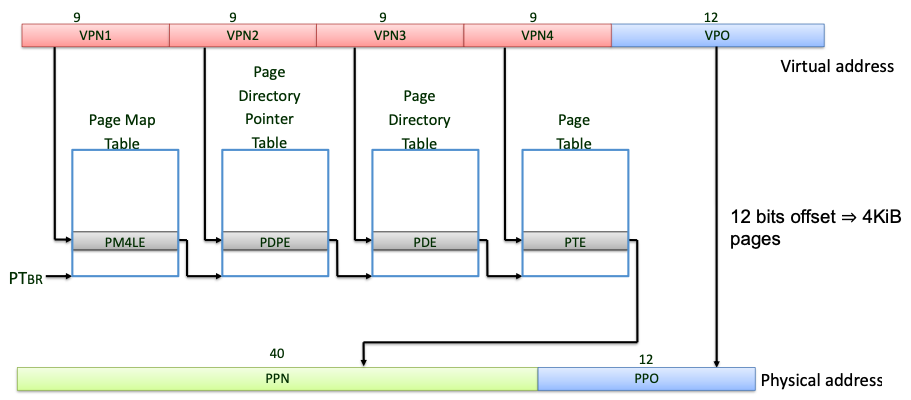
\includegraphics[width=\linewidth]{multi-level-pt.png}
\end{center}

On a context switch we need to store/restore the pointer to the page table and its size. One of the downsides of paging is if our page is very small and we do not need all of the space, this leads to internal fragmentation.


\subsection{Paged Segmentation}

It is possible to combine segmentation and paging. A paged segmentation memory management scheme is one where memory is addressed by a pair (segment.id, offset), as in a segmentation scheme, but each segment is itself composed of fixed-size pages whose page numbers are then translated to physical page numbers by a paged MMU.
\begin{center}
	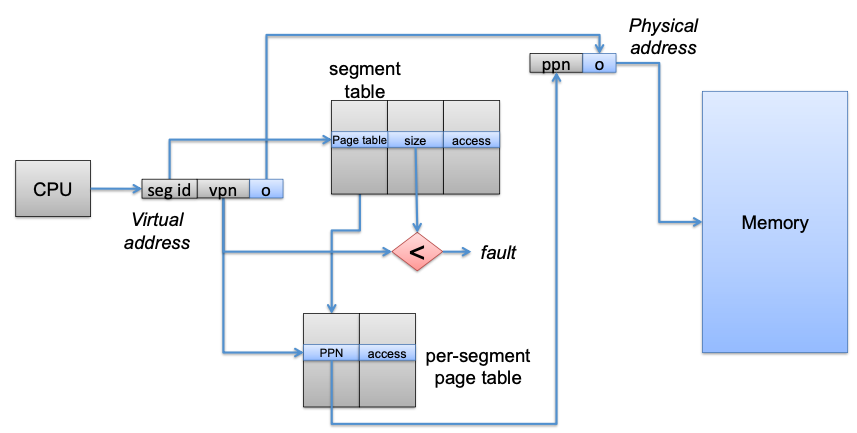
\includegraphics[width=\linewidth]{paged-segments.png}
\end{center}

One of the main benefits here is that each segment can have its own size of page table.


\subsection{Zero-on Reference}

The question how much physical memory is needed, is difficult to answer. So when a program runs out of memory, the system does the following:
\begin{enumerate}
	\item Page fault into OS kernel
	\item Kernel allocates some memory
	\item Zeroes the memory
	\item Modify page table
	\item Resume process
\end{enumerate}


\subsection{Fill On Demand}

Most programs do not need all their code to start running and might never use some code in its execution. Therefore we want to do something similar, we want to start a program before its code is in physical memory:
\begin{enumerate}
	\item Set all page table entries to invalid
	\item On first page reference, kernel trap
	\item Kernel brings page in from disk
	\item Resume execution
	\item Remaining pages can be transferred in the background while the program is running
\end{enumerate}


\subsection{Copy On Write}

Remember that we said \textit{fork()} copies the entire address space. This can be expensive and might not feasible in performance. On \textit{fork()} we copy the page table and set all mappings to read-only in both address spaces. Reads are now possible for both processes. If a write in either process causes a protection fault the kernel allocates a new frame and copies the referenced frames content into it. The faulting process now maps to the new copy and the protection changes to read/write (also for the non-faulting process).


\subsection{Managing Caches and the TLB}

\subsubsection{TLBs}

A problem with TLBs on context switches is that they can hold content inaccessible to the new process. To avoid having to flush the TLB, we introduce tags. Each TLB entry has a $6$-bit tag and the OS keeps track of a mapping between processes and tags. \medskip

\subsubsection{Caches}

\begin{center}
	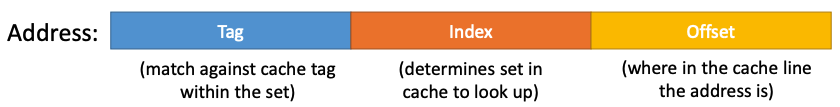
\includegraphics[width=\linewidth]{address.png}
\end{center}

Remember the different types of caches:
\begin{itemize}
	\item Virtually indexed, virtually tagged - simple and fast, but context switches are hard
	\item Physically indexed, physically tagged - can only be accessed after address translation
	\item Virtually indexed, physically tagged - overlap cache and TLB lookups
	\item Physically indexed, virtually tagged
\end{itemize}

Also remember the different write (write through, write back) and allocate (write allocate, non-write allocate) policies. In virtually tagged caches we can encounter homonyms, the same virtual address maps to multiple physical address spaces. To avoid this we can use physical tags, add address space identifiers, try to ensure disjoint address spaces or flush the cache on a context switch. \medskip

There is also a synonyms problem, where two virtual addresses map to the same physical address. This leads to inconsistent cache entries. The solutions to the homonym problem do not help here. To solve this problem we restrict VM mappings, so that synonyms map to the same cache set. 


\subsection{Demand Paging}

Demand paging solves the problem how to find a frame to use for missing pages. The goal is to minimize the page fault rate $p$ ($0 \leq p \leq 1$). The metric we are interested in is the effective access time $(1-p) * l_m + p * l_f$, where $l_m$ is the latency of a memory access and $l_p$ the latency of a page fault handling. Generally speaking the performance of a paging system depends on how many frames it has, but there is a diminishing return on adding new frames.

\subsubsection{Page Replacement Policies}

If a page has to be evicted, which one should be choose? We have already seen Least Recently Used (LRU) and First In First Out (FIFO). Both of these are not optimal, LRU is too expensive and FIFA works poorly for most workloads. A good compromise is the \textbf{Clock} or \textbf{2nd Chance} algorithm. It approximates LRU but much cheaper. It requires a linear table of all PFNs, with associated referenced bits. This can be best visualized as a circular buffer.
\begin{center}
	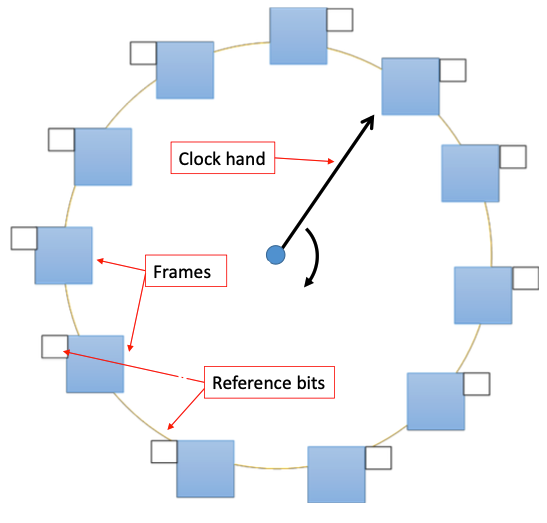
\includegraphics[width=0.8\linewidth]{2nd.png}
\end{center}

It works as follows:
\begin{itemize}
	\item Mark each frame when referenced for the first time
	\item If we want to replace a frame, process as follows: 
		\begin{itemize}
			\item If marked, unmark and advance the clock hand
			\item If unmarked, allocate this frame and mark it
		\end{itemize}
\end{itemize}

\subsubsection{Frame States}

\begin{center}
	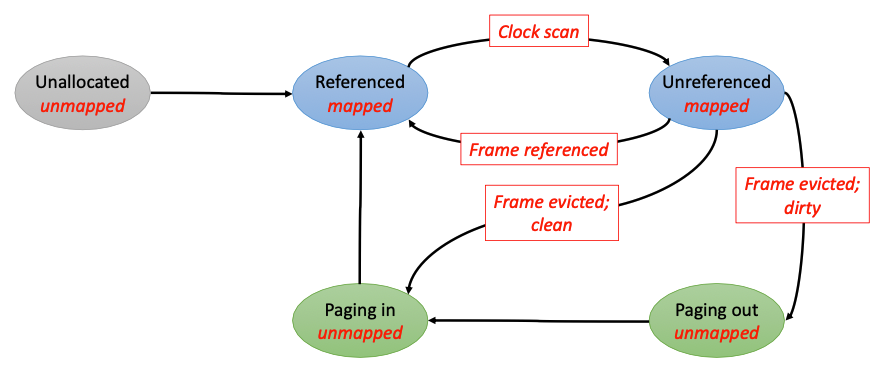
\includegraphics[width=\linewidth]{state_machine.png}
\end{center}

This only works if the corresponding bits are present in the page table and are properly set, in RISC-V for example these bits are present but do not have to be set. We can emulate these bits using faults.

\section{File System}


\subsection{Abstractions}

File systems are a very important concept and it makes sense to define an abstract file system. The main task of a file system is to virtualize, this means it should allow for multiplexing, have the same abstraction for multiple file systems implementation.

\subsubsection{Access Control}

We want to enforce some access control for our files. We call user or group of users a \textbf{principal} and files \textbf{objects}. One of the simplest way of representing this information would be in a matrix format. Each row would be a principal and columns correspond to objects. A entry in this matrix describes the rights the principal has in regards to the object. The problem with this idea is that such a matrix would become too large. \medskip

Another idea would be access control lists, a more compact representation. For each file you need to specify user and its access right, so you do not have to save any information on principals that do not have any rights to a file. If a new file gets created we use mandatory access control (MAC) to set the rights to a file. MAC defines the access policy centrally, so the principals cannot make policy decisions. This is easy to implement but hard to customize if you need special permissions. \medskip

A third idea would be to use capabilities, this means that there are tokens that give the holder of the token specific rights. \medskip

POSIX access control uses a hybrid approach. As principals there exist users but also groups. Access rights are divided into read, write and execute (\textit{rwx}). 

\subsubsection{File Abstraction}

Files consist of two parts. The first part is the \textbf{data}, consisting of unstructured bytes or blocks. The second part is the \textbf{metadata}, containing informations like type (structures or unstructured), time stamps, location, permissions, etc. The filename is not part of its metadata. \medskip

The filename is part of the \textbf{namespace}. Depending on the OS there are different restrictions on the filename, e.g. allowed characters. Filenames can be thought of as pointers to a file, meaning a file does not need a name or it could even have multiple names. The POSIX namespace results in a tree like structure, where each filename is preceded by the directories it is contained in. There are other location based bindings '.' meaning the current location and '..' being the parent directory. The challenge with this tree structure is to prevent cycles. \medskip

\subsubsection{File Descriptors}

\textbf{File descriptors} are used to open files and then perform operations on it. A file descriptor is basically an id that the OS give to a process to access a file (a FD comes with some metadata, e.g. type of access). Each processor has its own file descriptors. This concept is similar to capabilities. \medskip

There are different access types:
\begin{itemize}
	\item Direct - unrestricted access to the file without offset, curser starts at zero
	\item Sequential - access without rights to move the curser, writing happens at the end of the file
	\item Structured - defined agreement on how data gets written
\end{itemize}

\subsubsection{Memory-Mapped Files}

Alternatively, we can open files by mapping its content to virtual memory. This allows for anonymous memory, meaning we can treat memory regions as files even though this is not the case. It also allows us to have shared memory, by loading the same file on different processes. But if we use memory-mapped files, we have to take care of synchronisation between the memory and the file system.

\subsubsection{Executable Files}

Executing a file creates a new process, checks if the file is valid and then uses the ELF format to load the file and start execution.


\subsection{Implementations}

After having specified how an interface for a file system might look like, we know want to have a look at the implementations. \medskip

First we introduce an additional abstraction, \textbf{volumes}. A volume is a generic name for a storage device, consisting of a contiguous set of fixed-size blocks. To access blocks, we need \textbf{logical block addresses} (LBA), these are numbers for blocks on a volume. Closer to the hardware, there are \textbf{disk partitions}. Partitions are physical volumes divided into contiguous regions. For this to work we need to store a partition table at the start of the physical volume. \medskip

A file system implementation consists of a set of data structures. These are stored on a volume and allow for naming and protection. These things together form the \textbf{FS API}. \medskip

This API allows us to mount several file systems on top of each other. At the top we have the root file system and all other mount points are under the root (e.g. \textit{/dev/sda1}). \medskip

From the OS point of view, it implements a \textbf{virtual file system} layer in the kernel. This layer tries to resolve the type of file system that is being used. This allows for different file system implementations to coexist. \medskip

The main goals of concrete file system implementations depend on the device it is used on. Often they are a mixture of performance and reliability. In a typical file system implementation we will see the following things:
\begin{itemize}
	\item Directories and Indexes - where on the disk is the data for each file?
	\item Index Granularity - what is the unit of allocation for files?
	\item Free Space Maps - how to allocate more sectors on the disk?
	\item Locality Optimizations - how to make it go fast in the common case?
\end{itemize}

\subsubsection{The FAT File System}

FAT (file allocation table) is a very basic file system.
\begin{center}
	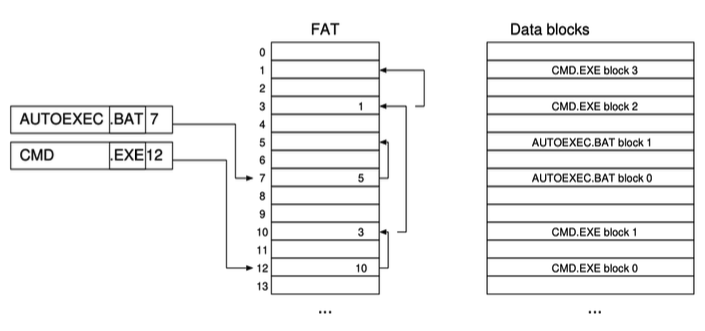
\includegraphics[width=0.9\linewidth]{fat.png}
\end{center}

For naming, the FAT system uses the filename and the extension. It then remembers the first block of that file. The file allocation table itself works like a linked list of blocks, where at the end of each block there is a pointer to the next block. To allocate new space, we simply need to scan the table. This can lead to very poor locality (fragmentation).

\subsubsection{The Berkeley Fast Filing System}

\begin{center}
	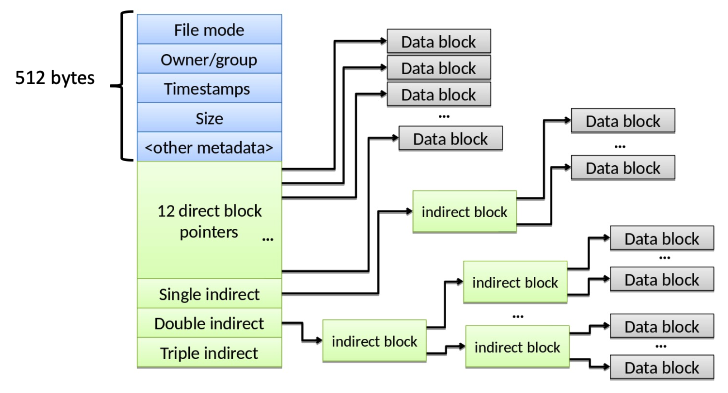
\includegraphics[width=0.8\linewidth]{bffs.png}
\end{center}

This system uses an index node (inode) for each file in the file system. The inode consists of the metadata and block pointers (or data directly if it fits). To allocate blocks it uses a bitmap indicating if a block is free or not. \medskip

Block groups are continuous subset of disk track  where related inodes, directories, free space map and file data blocks are gathered together. A superblock then holds all the informations about the overall layout and where the block groups are.

\subsubsection{Windows NTFS}

NTFS treats everything as a file, e.g. files system and file metadata. The master file table contains file entries for each file and is itself a file with the very first entry in the table. A MFT entry consists of metadata and a list of variable length attributes. One attribute is all the names for a file. If the data is small enough, it gets stored as part of the attributes, else it is stored in an extent. If works very similar to Berkeley FFS.

\begin{center}
	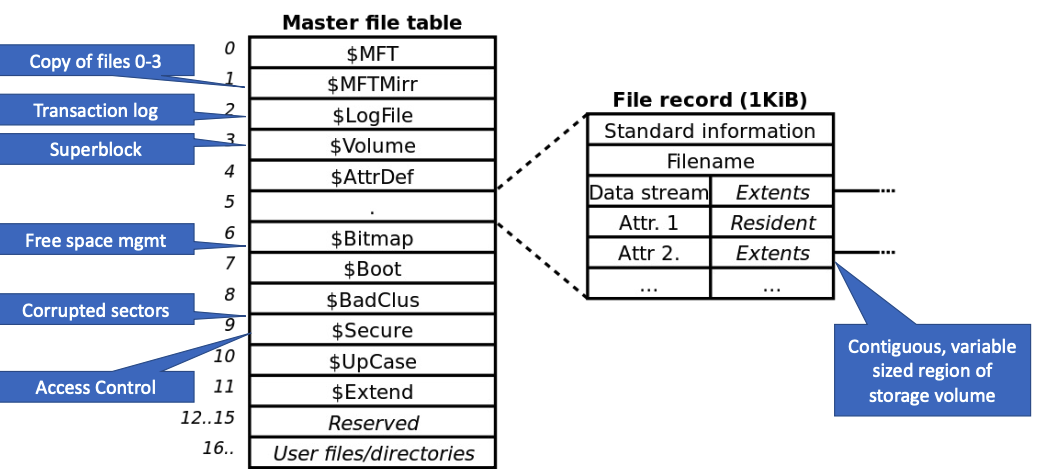
\includegraphics[width=\linewidth]{ntfs.png}
\end{center}

In NFTS file descriptors are basically pointers to extents. Additionally there are basic file descriptors.

\section{Network Stack}

In this part we want to look at what happens in the OS when we do networking on a low level. The role of the OS network stack is to handle all network related I/O. This includes delivering and transmitting packets, multiplex and demultiplex packets, and processing protocols. \medskip

The following parts play a role in the networking stack: 
\begin{itemize}
	\item the NIC (networking interface card) 
	\item first-level interrupt handlers
	\item NIC driver bottom half, e.g. deferred procedure calls
	\item NIC driver top half, kernel code
	\item app libraries, daemons, utils
\end{itemize}

Together they provide the following functionalities:
\begin{itemize}
	\item Multiplexing - taking packets from the user space, deciding the protocol to use and sending them out
	\item Encapsulation - taking raw data from an application and encapsulate it in a packet
	\item Protocol State Processing - advance the state of a protocol to process packets arriving
	\item Buffering and Data Movement - store data until the application decides to process it
\end{itemize}


\subsection{Header Space}

The header space is the set of all possible packet headers. The OS needs to process these headers as fast as possible and deliver them to the applications. Part of processing the header is to decide if the header is valid.


\subsection{Protocol Graphs}

Some OS maintain a protocol graph. The protocol graph of a network stack is the directed-graph representation of the forwarding and multiplexing rules. Nodes in the graph represent a protocol acting on a communication channel and perform de-/encapsulation and possibly de-/multiplexing. \medskip

If a node has multiple outgoing edges, it’s probably demultiplexing packets (vice versa for multiplexing). Note that this graph can well be cyclic due to tunnelling.


\subsection{Network I/O}

If the NIC receives a packet it copies it to a OS buffer, enqueues it on a descriptor ring and returns the buffer to the OS. If the OS wants to send a packet it enqueues it on a descriptor ring, notifies the NIC and after processing the NIC returns the buffer to the OS. A simplified implementation of the first-level- interrupt handler for packet receive looks as follows:

\begin{algorithm}[H]
\caption{First-level interrupt handler for receiving packets}
	\Comment{Inputs}
	\Comment{rxq: the receiver description queue}
	Acknowledge interrupt \\
	\While{not(rxq.empty())}{
	buf = rxq.dequeue() \\
	sk\_buf = sk\_buf\_allocate(buf) \\
	enqueue(sk\_buf) for processing \\
	post a DCP (software interrupt)
	}
	\Return
\end{algorithm}

Note that this only copies the packet and does not process it. This allows the OS to free the space for the NIC to receive new packets with deferring the processing the packet to later.


\subsection{Top-Half Handling}

In the top half of the stack, a socket interface is used: we can call \textit{bind(), listen(), connect(), send(), recv()} etc. from user space. \medskip

Some protocol processing happens in the kernel directly as a result of top half invocations, but for the most part the top half is concerned with copying network payload data and metadata between queues of protocol descriptors in the kernel and user-space buffers.


\subsection{Polling}

To increase performance, instead of the conventional interrupt-driven descriptor queues, a network receive queue can be serviced by a processor polling it contiguously. This eliminates the overhead of interrupts, context switches and maybe even kernel entry/exit. It requires a dedicated processor spinning, waiting for packets. \medskip

But even polling is insufficient to handle modern high- speed networks. It’s not clear how to scale this approach to multiple cores. Thus one relies on hardware support.


\subsection{Hardware Acceleration}

Today many operations are accelerated using dedicated hardware, e.g. by smart NICs. This works by having multiple physical queues for each connection. The OS then can bind an application to a hardware queue when needed. These smart NICs have dedicated hardware to perform operations on these queues, e.g. calculate checksums or applying filtering rules. \medskip

\textbf{RDMA} devices allow for direct memory accesses between different devices. This is extremely fast and specially useful in a datacenter context. On a downside allowing a remote devices to access a devices memory can be dangerous.


\subsection{Routing and Forwarding}

An OS also implements the core functionality of routers (forwarding and routing). For forwarding a set of hardware tables is used. Forwarding a packet on a receive queue essentially involves reading its header, then using this information to transfer the packet to one or more transmit queues to be sent. The forwarding tables are a result of the routing calculations, which mostly happen in user space.

\section{Virtual Machines}

A \textbf{virtual machine monitor} (VMM) virtualizes an entire system. The execution environment of the VMs we’ll look at provide a simulation of the raw machine hardware.\medskip

While a VMM is the functionality required to create the illusions of real hardware, the \textbf{hypervisor} is the software that runs on real, physical hardware and supports multiple VMs (each with its associated virtual machine monitor). There is one hypervisor on which many VMMs can run. We call a hypervisor running on bare metal a type-1 (native) hypervisor and one running on a real OS a type-2 (hosted) hypervisor. \medskip

OS-level virtualization uses a single OS to provide the illusion of multiple \textbf{containers} of that OS. Code running in a container have the same system call interface as the underlying OS, but cannot access any device. This is achieved by limiting the file system namespace (by changing the root for each container) and the process namespace, so processes can only see processes which share their container. In general, using containers is more efficient than using hypervisors.


\subsection{The Uses of Virtual Machines}

When multiple applications contend for resources the performance of one or more may degrade in ways outside the control of the OS. \textbf{Resource isolation} guarantees to one application that its performance will not be impacted by others, this is done by running the application in a VM. \medskip

\textbf{Cloud computing} is the business of renting computing resources as a utility to paying customers rather than selling hardware. They are primarily based on renting computing resources in the form of a VM (similar to resource isolation).

The term \textbf{server consolidation} refers to taking a set of services, each running on a dedicated server, and consolidating them onto a single physical machine so that each runs in a VM. \medskip

\textbf{Backward compatibility} is the ability of a new machine to run programs (including OSes) written for an old machine. \medskip


\subsection{Virtualizing the CPU}

To run an OS inside a VM, we need to completely virtualize the processor, including the kernel (else we simply could use threads). The processor in the VM clearly cannot execute a privileged instruction "for real". Instead, the default result is a trap/fault: \medskip

\textit{Trap-and-emulate} is a technique for virtualization which runs privileged code in non-privileged mode. Any privileged instruction causes a trap to the VMM, which then emulates the instruction and returns to the VM guest code.\medskip

The problem is that there might be some instructions which do not cause a trap when run in non-privileged mode but have a different behavior when executed in kernel mode (e.g. \textit{POPF} in x86). This cannot happen with a strictly virtualizable ISA. \medskip

An ISA is \textbf{strictly virtualizable} iff it can be perfectly emulated over itself with all non-privileged instructions executed naively and all privileged instructions emulated via traps. \medskip

There are different approaches to dealing with non strictly virtualizable ISA:
\begin{itemize}
	\item \textbf{Full software emulation}: Creates a virtual machine by interpreting all kernel-mode code in software. This is very slow, especially for many I/O operations.
	\item \textbf{Paravirtualization}: A paravirtualized guest OS is one which has been specifically modified to run inside a VM. Critical calls are replaced with explicit trap instructions.
	\item \textbf{Binary rewriting}: Scans compiled kernel code for unvirtualizable instructions and rewrites them – essentially patching the kernel on the fly. This is done on demand: All kernel pages are first protected and when first accessed (i.e., the pro- tection trap occurs), they get scanned and rewritten.	
	\item \textbf{Virtualization extensions}: Convert ISA by adding virtualization extensions. This typically takes the form of a new processor mode. Today, both ARM and x86 do have hardware support for virtualization.
\end{itemize}


\subsection{Viratualizing the MMU}

With virutalization, there is a second level of indirection with memory addresses. Now, a physical memory address is not unique in the machine, but in one VM (guest OS thinks it is physical). Thus, we define the \textbf{machine address} to be a real address on the machine which gets translated from the guest OSs physical address. From the view of the hypervisor, the machine address is the physical address.

\begin{center}
	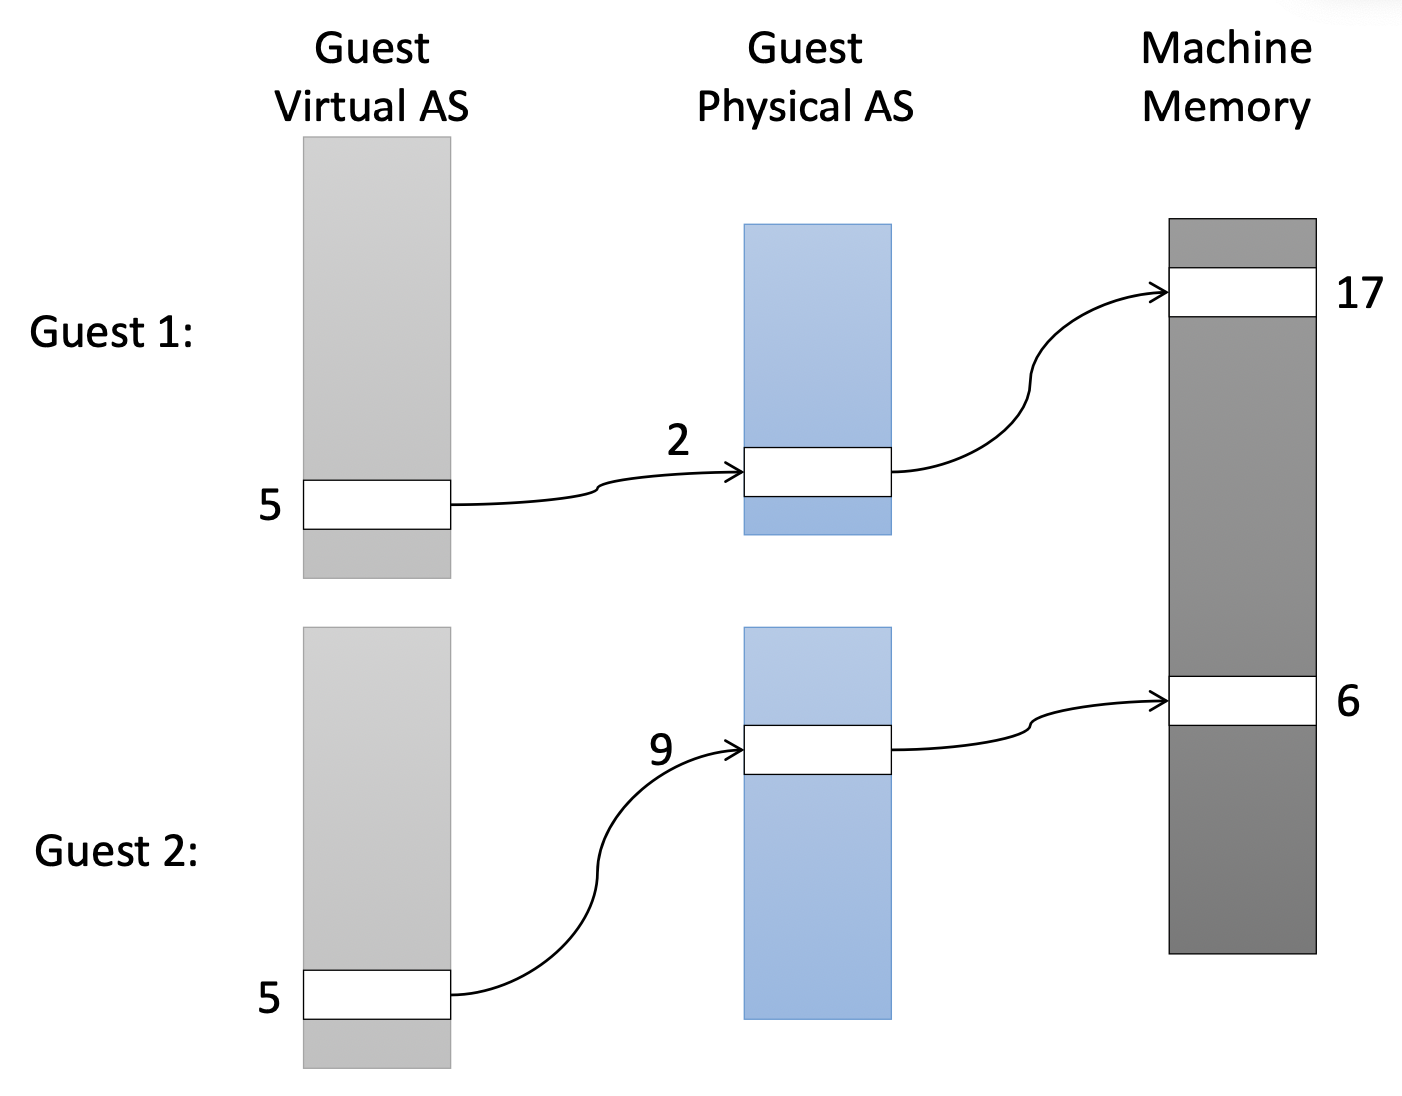
\includegraphics[width=0.8\linewidth]{virtual_mmu.png}
\end{center}

The hypervisor thus needs to translate a guest virtual address not to a guest physical address but to a machine address instead. There are several ways to do so:
\begin{itemize}
	\item Directly writable tables: The guest OS creates the page tables that the hardware uses to directly translate guest virtual to machine addresses. This requires paravirtualization. The VMM needs to check all writes to any PTE in the system. To change a PTBR, a hypercall is needed.
	\item A shadow page table is a page table maintained by the hypervisor which contains the result of translating virtual addresses through the guest OS’s page tables, and then the VMM’s physical-to-machine page table. The guest OS thus sets up its own PT, but they get never used. The VMM maintains the shadow PT which maps directly from guest VAs to machine addresses. \medskip
		
		The VMM must keep the shadow table consistent with both the guest’s PT and the hypervisors own physical-to-machine table. It achieves this by write-protecting all the guest OS's PT and trapping writes on them. When a write happens, it applies the update to the shadow page as well.
	\item Nested Paging/$2^{nd}$ level page translation is an enhancement to the MMU hardware that allows it to translate through two page tables (guest virtual to guest physical and guest physical to machine), caching the result (virtual to machine) in the TLB. This can be fast, but a TLB miss is costly.
\end{itemize}


\subsection{Viratualizing the Physical Memory}

How can the hypervisor allocate memory to a guest OS? The guest OS expects a fixed area of physical memory which does not change dynamically. In theory, this problem can be solved with paging. However, there is a phenomenon called \textbf{double paging}. Consider the following sequence of events:
\begin{enumerate}
	\item The hypervisor pages out a guest page $P$ to storage
	\item A guest OS decides to page out the virtual page associated with $P$ and touches it.
	\item This triggers a page fault in the hypervisor, hence $P$ gets paged back in memory.
	\item The page is immediately written out to disk and discarded by the guest OS.
\end{enumerate}
So to throw away a page in a guest OS, there are three I/O operations and one extra page fault! We could solve this problem with paravirtualization, but this introduces more complexity. \medskip

\textbf{Memory ballooning} is an elegant solution to this problem. It allows hypervisors to reallocate machine memory between VMs without incurring the overhead of double paging. A  device driver, the balloon driver, is installed in the guest kernel. This driver is VM-aware, i.e. it can make hypercalls and receive messages from the VMM. The principle is to block a large area of physical memory in the guest OS, which then can be allocated to the OS by unblocking it. \medskip

Memory can also be reclaimed from a guest OS (inflating the balloon):
\begin{enumerate}
	\item The VMM asks the balloon driver to return $n$ physical pages from the guest OS to the hypervisor.
	\item The balloon driver notifies the OS to allocate $n$ pages of memory for its private use.
	\item It communicates the guest-physical addresses of these frames to the VMM using a hypercall.
	\item The VMM unmaps these pages from the guest OS kernel and reallocates them elsewhere.
\end{enumerate}

Reallocating machine memory to the VM (deflating the balloon) can be done similarly:
\begin{enumerate}
	\item The VMM maps the newly allocate machine pages into guest-physical pages inside the balloon.
	\item The VMM then notifies the balloon driver that these pages are now returned.
	\item The balloon driver returns these guest-physical pages to the rest of the guest OS.
\end{enumerate}


\subsection{Viratualizing the Devices}

To software, a device is something that the kernel communicates using memory mapped I/O registers, interrupts from the device to the CPU and DMA access by the device to/from main memory. The hypervisor needs to virtualize all of this, too.\medskip

A device model is a software model of a device that can be used to emulate a hardware device, using trap-and-emulate to catch CPU writes to device registers. Interrupts from the emulated device are simulated using upcalls from the hypervisor into the guest OS kernel at its interrupt vector.\medskip

A \textbf{paravirtualized device} is a hardware device design which only exists as an emulated device. The driver of the device in the guest OS is aware that it is running in a VM and can communicate efficiently with the hypervisor using shared memory buffers and hypercalls.\medskip

For the device drivers talking to the real devices, we have the option to put them in the hypervisor kernel. Alternatively, one could use device passthrough, mapping a real hardware device into the physical address space of a guest OS. However, this does not solve the problem of sharing a real device among multiple virtualized guest OSes.\medskip

A \textbf{driver domain} is a virtual machine whose purpose it is to provide drivers for devices using device passthrough. With this, we can share devices across multiple VMs, by exporting a different to these devices using inter-VM communication channels. They are great for compatibility, but can be very slow, due to the communication overhead.\medskip

A \textbf{self-virtualizing} device is a hardware device which is designed to be shared be- tween different VMs by having different parts of the device mapped into each VM’s physical address space. \textbf{SR-IOV} is one form of this. \medskip

Single-Root I/O Virtualization (SR-IOV) is an extension to the PCIe standard which is designed to give VMs fast, direct but safe access to real hardware. An SR-IOV capable device appears initially as a single PCI device. This device can be configured to make further virtual functions appear in the PCI device space: each of this is a restricted version, but otherwise looks like a completely different, new device.


\subsection{Viratualizing the Network}

A soft switch is a network switch implementation inside a hypervisor which switches network packets sent from paravirtualized network interfaces in VMs to other VMs and/or one or more physical network interfaces.\medskip

The soft switch can be quite powerful but it needs to be fast. We can address a network interface inside a VM by giving each virtual network interface a MAC address on its own and letting DHCP do the rest.


\begin{center}
	\Large{\textbf{Distributed Systems}}
\end{center}

Today almost all computer systems are distributed, for different reasons:
\begin{itemize}
	\item Geography
	\item Parallelism - speed up computation
	\item Reliability - prevent data loss
	\item Availability - allow for access at any time, without bottlenecks, minimizing latency
\end{itemize}

Even though distributed systems have many benefits, such as increased storage or computational power, they also introduce challenging coordination problems.
\section{Fault Tolerance and Paxos}

In this section we want to create a fault-tolerant distributed system. We start out with a simple approach and improve our solution until we arrive at a system that works even under adverse circumstance, Paxos. \medskip

A \textbf{node} is a single actor in the system. In the message passing model we study distributed systems that consist of a set of nodes, where each node can perform local computations and send messages to every other node. Message loss means that there is no guarantee that a message will arrive safely at the receiver. This leads us to the first algorithm \medskip

\begin{algorithm}[H]
\caption{Naive Client-Server Algorithm}
	Client sends commands one at a time to server\\
	Server acknowledges every command\\
	If the client does not receive an acknowledgment within a reasonable time, it resends the command
\end{algorithm}

\medskip

This simple algorithm is the basis of many reliable protocols, e.g. TCP. The algorithm can easily be extended to work with multiple servers: The client sends each command to every server, and once the client received an acknowledgment from each server, the command is considered to be executed successfully. \medskip

In practice, messages might experience different transmission times, even if they are being sent between the same two nodes. A set of nodes achieves \textbf{state replication}, if all nodes execute a sequence of commands in the same order. Since state replication is trivial with a single server, we can desig- nate a single server as a serializer. \medskip

\begin{algorithm}[H]
\caption{State Replication with a Serializer}
	Client sends commands one at a time to the serializer\\
	Serializer forwards commands one at a time to all other servers\\
	Once the serializer received all acknowledgments, it notifies the client about the success
\end{algorithm}

\medskip

The downside of this algorithm is that the serializer is a single point of failure.

\subsection{Two-Phase Protocol}

\begin{algorithm}[H]
\caption{Two-Phase Protocol}
	\Comment{Phase 1}
	Client asks all servers for the lock \\
	\Comment{Phase 2}
	\eIf{client receives lock from every server}{
		Client sends command reliably to each server and gives the lock back
	}{
		Clients gives the received locks back \\
		Client waits, and then starts with Phase 1 again
	}
\end{algorithm}

\medskip

Instead of directly establishing a consistent order of commands, we can use a different approach: We make sure that there is always at most one client sending a command; i.e., we use mutual exclusion, respectively locking. \medskip

Still there are quite some problems with this algorithm. What happens if the node holding the locks crashes or it only gets part of the locks?

\subsection{Paxos}

A \textbf{ticket} is a weaker form of a lock, with the following properties:
\begin{itemize}
	\item Reissuable: A server can issue a ticket, even if previously issued tickets have not yet been returned.
	\item Ticket expiration: If a client sends a message to a server using a previously acquired ticket $t$, the server will only accept $t$, if it is the most recently issued ticket.
\end{itemize}

There is no more problem with crashes: If a client crashes while holding a ticket, the remaining clients are not affected. (At this point the naive ticket protocol is left out) \medskip

\begin{algorithm}[H]
\caption{Paxos Client / Proposer}
	\Comment{Initialization}
	$c$ 		\tcc*[f]{command to execute}\\
	$t = 0$ 	\tcc*[f]{ticket number to try}\\
	
	\BlankLine
	\Comment{Phase 1}
	$t = t + 1$\\
	Ask all servers for ticket $t$
	
	\BlankLine
	\Comment{Phase 2}
	\If{a majority answers ok}{
		Pick($T_{store}, C$) with largest $T_{store}$
		\If{$T_{store} > 0$}{
			$c = C$
		}
		Send propose($t, c$) to same majority
	}
	
	\BlankLine
	\Comment{Phase 3}
	\If{a majority answers success}{
		Send execute($c$) to every server
	}
\end{algorithm}

\medskip

\begin{algorithm}[H]
\caption{Paxos Server / Acceptor}
	\Comment{Initialization}
	$T_{max} = 0$ 	\tcc*[f]{largest issued ticket}\\
	$C = \bot$ 		\tcc*[f]{stored command}\\
	$T_{store} = 0$ 	\tcc*[f]{ticket used to store $C$}\\
	
	\BlankLine
	\Comment{Phase 1}
	\If{$t > T_{max}$}{
		$T_{max} = t$\\
		Answer with ok($T_{max}, C$)
	}
	
	\BlankLine
	\Comment{Phase 2}
	\If{$t = T_{max}$}{
		$C = c$\\
		$T_{store} = t$\\
		Answer success
	}
	
\end{algorithm}

\medskip

Unlike previously mentioned algorithms, there is no step where a client explicitly decides to start a new attempt and jumps back to Phase 1. This has the advantage that we do not need to be careful about selecting “good” values for timeouts, as correctness is independent of the decisions when to start new attempts. The performance can be improved by letting the servers send negative replies in Phase 1 or 2 if the ticket expired. Using randomized backoff we can eliminate contention between clients. \medskip

\textbf{Theorem:} If a command c is executed by some servers, all servers (eventually) execute c. \medskip

Note that Paxos cannot make progress if half (or more) of the servers crash, as clients cannot achieve a majority anymore. \medskip

For state replication we need to be able to execute multiple commands, we can extend each instance with an instance number, that is sent around with every message. Once the 1st command is chosen, any client can decide to start a new instance and compete for the 2nd command. If a server did not realize that the 1st instance already came to a decision, the server can ask other servers about the decisions to catch up.

\section{Consensus}


\subsection{Two Friends}

A protocol used in a network with unreliable connections that relies on ACKing might not terminate: If $A$ sends to $B$ and expects an ACK, $B$ also needs $A$ to ACK the ACK message and so on. This cannot terminate.


\subsection{Consensus}

There are $n$ nodes, $f$ of which might crash. $n-f$ nodes are correct. Each node $i$ starts with an input $v_i$. All nodes must decide on one of those values, satisfying the following:
\begin{itemize}
	\item \textbf{Agreement}: all correct nodes decide for the same value
	\item \textbf{Termination}: all correct nodes terminate in finite time
	\item \textbf{Validity}: the decision value must be the input value of some node
\end{itemize}

We assume that the links are reliable and that each node can send to each other node. However there is no broadcast, a node can only send individual messages. If we study Paxos carefully, we will notice that \textbf{Paxos does not guarantee termination}.


\subsection{Impossibility of Consensus}

We restrict the input values to be either 0 or 1. Even with this simplification, there is no algorithm which solves the consensus problem. \medskip

In the \textbf{asynchronous model}, algorithms are event based (upon receiving msg, do ...). Nodes cannot access a synchronous clock. A message from a node to another will arrive in finite but unbounded time. This is a formalization of the variable message delay model. \medskip

For algorithms in the asynchronous model, the \textbf{runtime} is the number of time units from the start of the execution to its completion in the worst case (assuming a delay of at most one time unit). \medskip

We say that a system is \textbf{fully defined} (at any point during the execution) by its configuration $C$. The configuration includes the state of every node, and all messages that are in transit. A configuration if \textbf{univalent}, if the decision value is determined independently of what happens afterwards, else we call it \textbf{bivalent}. We might also call a configuration that is univalent for a value $v$ $v$-valent.\medskip

\textbf{Lemma:} There is at least one selection of input values $V$ such that the according initial configuration $C_0$ is bivalent, if $f > 1$. (We are gonna omit the proofs) \medskip

A \textbf{transition} from configuration $C$ to a following configuration $C_\tau$ is characterized by an event $\tau = (u, m)$, where node $u$ receives a message $m$. \medskip

The \textbf{configuration tree} is a directed tree of configurations. Its root is $C_0$ which is fully characterized by the input values $V$. The edges of the tree are transitions; every configuration has all applicable transitions as outgoing edges. Leaves are terminal configurations. \medskip

\textbf{Lemma:} Assume two transitions $\tau_1, \tau_2$ for $u_1 \neq u_2$ which are both applicable to $C$. It holds that $C_{\tau_1 \tau_2} = C_{\tau_2 \tau_1}$. \medskip

A configuration is \textbf{critical} if $C$ is bivalent, but all configurations that are direct children of $C$ are univalent. Informal we can say that $C$ is the last moment in the execution where the decision is not yet taken. \medskip

\textbf{Lemma:} If a system is in a bivalent configuration, it must reach a critical configuration within finite time, or it does not always solve consensus. \medskip

\textbf{Lemma:} If a configuration tree contains a critical configuration, crashing a single node can create a bivalent leaf.\medskip

From these lemmas we derive that there is no deterministic algorithm which always achieves consensus in the asynchronous model, while $f > 0$. If $f = 0$ all nodes can simply send their value to all other nodes and then choose the minimum.


\subsection{Randomized Consensus}

As there exists no deterministic solution, we use randomness. In the following we assume $f < n/2$. \medskip

The basic idea of a possible algorithm is that each node chooses $v_i$ at random until a majority gets the same resulting value.\medskip

\begin{algorithm}[H]
\caption{Randomized Consensus (Ben-Or)}
	$v_i \in [0, 1]$ 		\tcc*[f]{input bit}\\
	round = 1 \\
	decided = false \\
	
	\BlankLine
	Broadcast myValue($v_i$, round) \\
	\BlankLine
	
	\While{true} {
		\BlankLine
		\Comment{Propose}
		\BlankLine
		
		Wait until a majority of myValue messages of the current round arrived \\
		\eIf{all messages have the same value $v$}{
			Broadcast propose($v$, round)
		}{
			Broadcast propose($\bot$, round)
		}
		
		\BlankLine
		\If{decided}{
			Broadcast myValue ($v_i$, round+1) \\
			Decide for $v_i$ and terminate
		}
		
		\BlankLine
		\Comment{Vote}
		\BlankLine
		
		Wait until a majority of propose messages of current round arrived \\
		\eIf{all message propose the same value $v$}{
			$v_i = v$ \\
			decided = true
		}{
			\eIf{there is at least on proposal for $v$}{
				$v_i = v$
			}{
				Choose $v_i$ randomly, with Pr$[v_i = 0]$ = Pr$[v_i = 1] = 1/2$ 
			}
		}
		
		round += 1 \\
		Broadcast myValue($v_i$, round)
	}
\end{algorithm}
\medskip

As long as no node decides and terminates, the algorithm will never get stuck, independent of which nodes crash. Further the algorithm satisfies the validity, the agreement and the termination requirement (expected $\mathcal{O}(2^n)$). \medskip

There is no consensus algorithm for the asynchronous model that tolerates $f \geq n/2$. \medskip

We have seen that the algorithm solves consensus with optimal fault-tolerance – but it is awfully slow. The reason for this is the individual coin tossing. We can improve this by tossing a so-called shared coin.


\subsection{Shared Coin}

Instead of picking each value with probability $1/2$, we use the shared coin to introduce randomness. \medskip

\begin{algorithm}[H]
\caption{Shared Coin}
	Choose local coin $c_u = 0$ with probability $1/n$, else $c_u =1$ \\
	Broadcast myCoin($c_u$) \\
	
	\BlankLine
	Wait for $n-f$ coins and store them in a local coin set $C_u$ \\
	Broadcast myCoinSet($C_u$) \\
	
	\BlankLine
	Wait for $n-f$ coin sets \\
	\eIf{at least one coin is 0 among all coins in the coin sets}{
		return 0
	}{
		return 1
	}
\end{algorithm}
\medskip

If $f < n/3$, the algorithm implements a shared coin. Plugging this into our randomized algorithm, we get a consensus algorithm which terminates in a constant expected number of rounds tolerating up to $f < n/3$ crash failures.

\section{Byzantin Agreement}

In some sort, byzantine agreement is the generalization of consensus. A node which can have arbitrary behavior is called byzantine. This includes sending wrong messages, different messages to different neighbors lying about input values and crashing. \medskip

Fining consensus in a system with byzantine nodes is called \textbf{byzantine agreement}. An algorithm is $f$-resilient if it still works correctly with $f$ byzantine nodes. If a algorithms solves the byzantine agreement, it solves consensus, too. \medskip

For an byzantine agreement, we need agreement, termination and validity. While the first two aspects are defined as before, validity is not that straight-forward.


\subsection{Validity}

There are four possible definitions for validity:
\begin{itemize}
	\item \textbf{Any-Input Validity} - The decision value must be the input of any node. This does not make sense for byzantine nodes, as they can lie about their inputs.
	\item \textbf{Correct-Input Validity} - The decision value must be the input of a correct node.
	\item \textbf{All-Same Validity} - If all nodes start with the same input value, the decision value must be this input value.
	\item \textbf{Median Validity} - If the input values are orderable, byzantine outliers can be prevented by agreeing on a value close to the median of the correct input values. How close depends on the number of byzantine nodes $f$.
\end{itemize}

First, we will only look at the synchronous model, where nodes operate in synchronous rounds. In each round, each node may send a message, receive messages, and do some local computation. For algorithms in the synchronous model, the runtime is simply the number of rounds from the start of the execution to its completion in the worst case.


\subsection{How Many Byzantine Nodes?}

\begin{algorithm}[H]
\caption{Byzantine Agreement with $f = 1$ }
	Code for node $u$, with input value $x$ \\
	
	\BlankLine
	\Comment{Round 1}
	\BlankLine
	
	Send tuple($u,x$) to all other nodes \\
	Receive tuple($v, y$) from all other nodes \\
	Store all received tuples in a set $S_u$
	
	\BlankLine
	\Comment{Round 2}
	\BlankLine
	
	Send set $S_u$ to all other nodes \\
	Receive sets $S_v$ from all nodes $v$ \\
	$T$ = set of tuples seen in at least two sets $S_v$, including own $S_u$ \\
	Let $y$ be the smallest value in $T$ \\
	Decide on value $y$
\end{algorithm}
\medskip

If a byzantine node does not follow the protocol, it can be easily detected and its messages discarded. However, if it sends syntactically correct messages, bad things might happen, e.g. if a byzantine node sends different values to different nodes in the first round. \medskip

If $n \geq 4$, all nodes have the same set $T$. Thus, each one will see every correct value twice. So all correct values are in $T$. Based on this insight, we can show that this algorithm solves byzantine agreement for $n \geq 4$. \medskip

Further we can show that three nodes cannot reach byzantine agreement and that a larger network cannot reach byzantine agreement for $f \geq n / 3$ byzantine nodes.


\subsection{The King Algorithm}

\begin{algorithm}[H]
\caption{King Algorithm for $f < n / 3$}
	$x$ = my input value \\
	\For{phase = 1 to f + 1}{
		\BlankLine
		\Comment{Vote}
		\BlankLine
		
		Broadcast value($x$)
		
		\BlankLine
		\Comment{Propose}
		\BlankLine
		
		\If{value(y) received at least n − f times}{
			Broadcast propose($y$)
		}
		
		\If{propose(z) received more than f times}{
			$x = z$
		}
		
		\BlankLine
		\Comment{King}
		\BlankLine
		
		Let node $v_i$ be the predefined king of  phase $i$ \\
		The king $v_i$ broadcasts its current value $w$ \\
		\If{received strictly less than n - f propose(y)}{
			$x = w$
		}
	}
\end{algorithm}
\medskip

This algorithm fulfils the all-same validity. Further if a correct node proposes $x$, no other correct nodes proposes $y \neq x$, if $n > 3f$. \medskip

\textbf{Lemma:} There will be at least one phase with a correct king. \medskip

Also, after a round with a correct king, the correct nodes will not change their values anymore. Using all this facts, it’s easy to show that this algorithm solves the byzantine agreement. However, the algorithm needs $f + 1$ predefined kings. If they are not given beforehand, finding those kings is a byzantine agreement task by itself, so this must be done before the King algorithm. \medskip

A synchronous algorithm solving consensus in the presence of $f$ crashing nodes needs at least $f + 1$ rounds, if the nodes decide for the minimum value. Since byzantine nodes can also just crash, this lower bound also holds for byzantine agreement, so our algorithm has an asymptotically optimal runtime.


\subsection{Asynchronous Byzantine Agreement}

What if the nodes only work in a asynchronous manner? \medskip

\begin{algorithm}[H]
\caption{Asynchronous Byzantine Agreement (Ben-Or for $f < n/10)$}
	$x_u \in \{0,1\}$ \\
	round = 1
	
	\BlankLine
	
	\While{true}{
		Broadcast propose($x_u$, round) \\
		Wait until $n - f$ propose messages of current round arrived \\
		
		\BlankLine
		
		\eIf{at least n/2 + 3f + 1 propose messages contain same value x}{
			Broadcast propose($x$, round + 1) \\
			Decide for $x$ and terminate
		}{
			\eIf{at least n/2 + f + 1 propose messages contain same value x}{
				$x_u = x$
			}{
				choose $x_u$ randomly with prob. $1/2$
			}
		}
		
		\BlankLine
		
		round += 1	
	}
	
\end{algorithm}
\medskip

If a correct node chooses $x$ in line 11, then no other correct node chooses a value $y \neq x$ in line 11. The algorithm above solves binary byzantine agreement for up to $f < n/10$. There are other algorithms for asynchronous byzantine agreement which tolerate up to $f < n/3$. Nearly all developed algorithms for byzantine agreement (both synchronous and asynchronous) only satisfy all-same validity, with some exceptions.


\subsection{Random Oracle and Bitstring}

A \textbf{random oracle} is a trusted (non-byzantine) random source which can generate random values. \medskip

In the previous algorithm, replace line 13 by "return $c_i$, where $c_i$ is $i$-th random bit by oracle". So instead of every node throwing a local coin (and hoping that they all show the same), the nodes will base their random decision on the proposed algorithm. Using this, we could solve asynchronous byzantine agreement in expected constant number of rounds. \medskip

Unfortunately, random oracles do not really exist in the world. We thus try to use random bitstrings to simulate the behavior of a random oracle: this is a string of random binary values known to all participating nodes when starting a protocol. So in line 13 we choose the $i$-th bit in the random bitstring. But is this really random? Not quite! As the string is known beforehand, byzantine nodes know in the $i$-th step of a protocol the value $c_{i+1}$. Thus the algorithm might not terminate.

\section{Broadcast and Shared Coin}

Our asynchronous byzantine agreement solution is awfully slow or has unrealistic assumptions. Can we at least solve asynchronous (assuming worst-case scheduling) consensus if we have crash failures?


\subsection{Shared Coin on Blackboard}

The \textbf{blackboard} is a trusted authority which supports two operations. A node can \textbf{write} its message to the blackboard and a node can \textbf{read} all the values from that have been written to the blackboard so far. We assume that the nodes cannot reconstruct the order in which the messages are written to the blackboard since the system is asynchronous. \medskip

\begin{algorithm}[H]
\caption{Crash-Resilient Shared Coin with Blackboard}
	\While{true}{
		Choose new local coin $c_u$ with 
		$$c_u = \begin{cases}
			1  & \text{with probability } 1/2 \\
			-1 & \text{with probability } 1/2
		\end{cases}$$
		
		Write $c_u$ to the blackboard \\
		Set $C = $ read all coins on the blackboard \\
		\If{$|C| \geq n^2$}{
			\Return sign(sum($C$))
		}
	}
\end{algorithm}
\medskip

This is a wait-free algorithm that works even for a worse-case scheduler for crashing nodes. A single node can single- handedly generate all $n^2$ coinflips, without waiting. However, it does not work for byzantine nodes, as such a node could write in rapid succession at the beginning. \medskip

Assuming a trusted blackboard does not seem practical. However, fortunately, we can use advanced broadcast methods in order to implement something like a blackboard with just messages.


\subsection{Broadcast Abstractions}

A message received by a node $v$ is called \textbf{accepted} if node $v$ can consider this message for its computation. \textbf{Best-effort broadcast} ensures that a message that is sent from a correct node $u$ to another correct node $v$ will eventually be received and accepted by $v$. \medskip

\textbf{Reliable broadcast} ensures that the nodes eventually agree on all accepted messages. That is, if a correct node $v$ considers message $m$ as accepted, then every other node will eventually consider message $m$ as accepted. The following algorithm satisfies this definition: \medskip

\begin{algorithm}[H]
\caption{Asynchronous Reliable Broadcast}
	Broadcast own message msg$(u)$ \\
	\textbf{upon} receiving msg$(v)$ from $v$ or echo$(w, msg(v))$ from $n - 2f$ nodes $w$: \\
	Broadcast echo$(u$, msg$(v)$\\
	\textbf{end upon} \\
	
	\textbf{upon} receiving echo$(w, msg(v))$ from $n - f$ nodes $w$: \\
	Accept msg$(v)$\\
	\textbf{end upon}
\end{algorithm}
\medskip

This algorithm satisfies the following three properties:
\begin{itemize}
	\item If a correct node broadcasts a message reliably, it will eventually be accepted by every other correct node.
	\item If a correct node has not broadcast a message, it will not be accepted by any other correct node.
	\item If a correct node accepts a message, it will be eventually accepted by every correct node.
\end{itemize}

This algorithm can tolerate $f < n/3$ byzantine nodes or $f < n/2$ crash failures. \medskip

It only makes sure that all messages of correct nodes will be accepted \textit{eventually}. This algorithm allows byzantine nodes to issue arbitrarily many messages, which may result in problems for protocols where each node is only allowed to send one message per round. \medskip

\textbf{FIFO reliable broadcast} defines an order in which the messages are accepted in the system. If a node $u$ broadcasts message $m_1$ before $m_2$, than any node $v$ will accept $m_1$ before $m_2$. \medskip

\begin{algorithm}[H]
\caption{FIFO Reliable Broadcast}
	Broadcast own round $r$ message msg$(u, r)$ \\
	\textbf{upon} receiving first msg$(v, r)$ from $v$ for round $r$ or echo$(w, msg(v, r))$ from $n - 2f$ nodes $w$: \\
	Broadcast echo$(u$, msg$(v, r)$\\
	\textbf{end upon} \\
	
	\textbf{upon} receiving echo$(w, msg(v, r))$ from $n - f$ nodes $w$: \\
	\If{accepted msg$(v, r-1)$}{
			Accept msg$(v, r)$
	}
	\textbf{end upon}
\end{algorithm}
\medskip

This algorithm can tolerate $f < n/5$ byzantine nodes or $f < n/2$ crash failures. Further it only only accepts one message per node. \textbf{Atomic broadcast} makes sure that all messages are accepted in the same order by every node. Now we finally have all tools to solve asynchronous consensus.


\subsection{Blackboard with Message Passing}

\begin{algorithm}[H]
\caption{Crash-Resilient Shared Coin}
	\While{true}{
		Choose new local coin $c_u$ with 
		$$c_u = \begin{cases}
			1  & \text{with probability } 1/2 \\
			-1 & \text{with probability } 1/2
		\end{cases}$$
		
		FIFO-broadcast coin($c_u, r$) to all nodes \\
		Save all received coins $coin(c_v , r)$ in a set $C_u$ \\
		Wait until accepted own coin$(c_u)$ \\
		Request $C_v$ from $n - f$ nodes $v$, and add newly seen coins to $C_u$ \\
		\If{$|C_u| \geq n^2$}{
			\Return sign(sum($C_u$))
		}
	}
\end{algorithm}
\medskip

This solves asynchronous binary agreement for $f < n/2$ crash failures. But what about byzantine agreement? We need even more powerful methods!


\subsection{Using Cryptography}

Let $t, n \in \N$ with $1 \leq t \leq n$. An algorithm that distributes a secret among $n$ participants such that $t$ participants need to collaborate to recover the secret is called a $(t, n)$-\textbf{threshold secret sharing scheme}. \medskip

Every node can \textbf{sign} its messages in a way that no other node can forge, thus nodes can reliably determine which node a signed message originated from. We denote a message $x$ signed by node $u$ with msg$(x)_u$.

Those methods allow us to create an algorithm like this: \medskip

\begin{algorithm}[H]
\caption{$(t, n)$-Treshold Secret Sharing}
	Input: A secret $s$, represented as a real number 
	
	\BlankLine
	\Comment{Secret distribution by dealer $d$}
	\BlankLine
	
	Generate $t-1$ random numbers $a_1, ..., a_{t-1} \in \R$ \\
	Obtain a polynomial $p$ of degree $t-1$ with $$p(x) = s + a_1x + ... + a_{t-1}x^{t-1}$$ \\
	Generate $n$ distinct $x_1, ..., x_n \in \R \backslash \{0\}$ \\
	Distribute share msg$(x_1, p(x_1))_d$ to node $v_1, ...,$ msg$(x_n, p(x_n))_d$ to node $v_n$ 
	
	\BlankLine
	\Comment{Secret recovery}
	\BlankLine
	
	Collect $t$ shares msg$(x_u,p(x_u))_d$ from at least $t$ nodes \\
	Use Lagrange's interpolation formula to obtain $p(0) = s$
	
\end{algorithm}
\medskip

This algorithm relies on a trusted dealer who cannot by byzantine and creates the polynomial. Further the communication between the dealer and the nodes must be private, i.e., a byzantine party cannot see the shares sent to the correct nodes. Using an $(f + 1, n)$-threshold secret sharing scheme, we can encrypt messages in such a way that byzantine nodes alone cannot decrypt them. This allows us to solve byzantine agreement for $f < n/10$ in expected $3$ number of rounds. \medskip

A\textbf{ hash function} $U \mapsto S$ is called \textbf{cryptographic}, if for a given $z \in S$ it is computationally hard to find an element $x \in U$ with hash$(x) = z$. Examples are the Secure Hash Algorithm (SHA) and the Message-Digest Algorithm (MD). With cryptographic hashing, we can implement a synchronous byzantine shared coin: \medskip

\begin{algorithm}[H]
\caption{Simple Synchronous Byzantine Shared Coin }
	Each node has a public key that is known to all nodes \\
	Let $r$ be the current round of Alg. 11 \\
	Broadcast msg$(r)_u$, i.e., round number $r$ signed by node $u$ \\
	Compute $h_v =$ hash(msg$(r)_v$) for all received messages msg$(r)_v$ \\
	Let $h_{min} = \min_v h_v$ \\
    \Return least significant bit of $h_{min}$
\end{algorithm}
\medskip

This algorithm plugged into Alg. 11 solves synchronous byzantine agreement in expected $3$ rounds (roughly) for up to $f < n/10$ byzantine failures.

\section{Consistency and Logical Time}

This section involves concepts already seen in Parallel Programming and DMDB.


\subsection{Consistency Models}

An \textbf{object} is a variable or a data structure storing information. Object is a general term for any entity that can be modified. An \textbf{operation} $f$ accesses or manipulates an object. The operation $f$ starts at wall-clock time $f_*$ and ends at wall-clock time $f_\dagger$. If $f_\dagger < g_*$ we simply write $f < g$. \medskip

An \textbf{execution} $E$ is a set of operations on one or multiple objects that are executed by a set of nodes. An execution restricted to a single node is a \textbf{sequential execution}. This means that no two operations $f$ and $g$ are concurrent, i.e., we have $f < g$ or $g < f$. \medskip

Two executions are \textbf{semantically equivalent} if they contain exactly the same operations. Moreover, each pair of corresponding operations has the same effect in both executions. \medskip

An execution $E$ is called \textbf{linearizable} (or atomically consistent), if there is a sequence of operations (sequential execution) $S$ such that:
\begin{itemize}
	\item $S$ is correct and semantically equivalent to $E$
	\item Whenever $f < g$ for two operations $f,g$ in $E$, then also $f < g$ in $S$
\end{itemize}

A linearization point of operation $f$ is some $f_\circ \in [f_* , f_\dagger]$. $E$ is linearizable if and only if there exist linearization points such that the sequential execution $S$ that results in ordering the operations according to those linearization points is semantically equivalent to $E$. \medskip

An execution $E$ is called \textbf{sequentially consistent}, if there is a sequence of operations $S$ such that:
\begin{itemize}
	\item $S$ is correct and semantically equivalent to $E$
	\item Whenever $f < g$ for two operations $f,g$ on the same node in $E$, then also $f < g$ in $S$
\end{itemize}
Every linearizable execution is also sequentially consistent.
$$\text{linearizability} \implies \text{sequential consistency}$$

An execution $E$ is called \textbf{quiescently consistent}, if there is a sequence of operations $S$ such that:
\begin{itemize}
	\item $S$ is correct and semantically equivalent to $E$
	\item Let $t$ be some quiescent point, i.e., for all operations $f$ we have $f_\dagger < t$ or $f_* > t$. Then for every $t$ and every pair of operations $g, h$ with $g_\dagger < t$ and $h_* > t$ we also have $g<h$ in $S$
\end{itemize}
Every linearizable execution is also quiescently consistent.
$$\text{linearizability} \implies \text{quiescently consistency}$$

However, sequentially consistent and quiescent consistency do not imply one another. A system or an implementation is called linearizable if it ensures that every possible execution is linearizable. Analogous definitions exist for sequential and quiescent consistency. \medskip

Let $E$ be an execution involving operations on multiple objects. For some object $o$ we let the \textbf{restricted execution} $E|o$ be the execution $E$ filtered to only contain operations involving object $o$. \medskip

A consistency model is called \textbf{composable} if the following holds: If for every object $o$ the restricted execution $E|o$ is consistent, then also $E$ is consistent. Sequential consistency is not composable, but linearizability is.


\subsection{Logical Clocks}

To capture dependencies between nodes in an implementation, we can use logical clocks. These are supposed to respect the so-called happened-before relation. \medskip

Let $S_u$ be a sequence of operations on some node $u$ and define $\to$ to be the \textbf{happened-before relation} on $E := S_1 \cup ... \cup S_n$ that satisfies the following three conditions:
\begin{enumerate}
	\item If a local operation $f$ occurs before operation $g$ on the same node (i.e. $f < g$), then $f \to g$
	\item If $f$ is a send operation of one node and $g$ is the corresponding receive operation of another node, then $f \to g$
	\item If $f, g, h$ are operations such that $f \to g, g \to h$ then also $f \to h$
\end{enumerate}
If for two distinct operations $f,g$ neither $f \to g$ nor $g \to f$, then we also say $f$ and $g$ are independent and write $f \sim g$. Sequential computations are characterized by $\to$ being a total order, whereas the computation is entirely concurrent if no operations $f,g$ with $f \to g$ exist. \medskip

An execution $E$ is called \textbf{happened-before consistent}, if there is a sequence of operations $S$ such that:
\begin{itemize}
	\item $S$ is correct and semantically equivalent to $E$
	\item Whenever $f \to g$ in $E$, then also $f<g$ in $S$
\end{itemize}

This is actually an equivalent definition to sequential consistency. \medskip

A \textbf{logical clock} is a family of functions $c_u$ that map every operation $f \in E$ on node $u$ to some logical time $c_u(f)$ such that the happened-before relation is respected, i.e., for two operations $g$ on node $u$ and $h$ on node $v$:
$$g \to \implies c_u(g) < c_u(h)$$

If the reverse implication also holds, then the clock is called a \textbf{strong logical clock}. \medskip

\begin{algorithm}[H]
\caption{Lamport Clock}
	Initialize $c_u := 0$ \\
	Upon local operation: Increment current local time $c_u := c_u + 1$ \\
	Upon send operation: Increment $c_u := c_u + 1$ and include $c_u$ as $T$ in message \\
	Upon receive operation: Extract $T$ from message and update $c_u := \max (c_u,T) + 1$
\end{algorithm}
\medskip

This is not an implementation of a strong log- ical clock. To achieve this, nodes also have to gather information about other clocks in the system. We can do this with \textbf{vector clocks}: \medskip

\begin{algorithm}[H]
\caption{Lamport Clock}
	Initialize $c_u[v] := 0$ for all other nodes $v$ \\
	Upon local operation: Increment current local time $c_u[u] := c_u[u] + 1$ \\
	Upon send operation: Increment $c_u[u] := c_u[u] + 1$ and include the vector $c_u$ as $d$ in message \\
	Upon receive operation: Extract vector $d$ from message and update $c_u[v] := \max (d[v], c_u[v])$ for all entries $v$. Increment $c_u[u] := c_u[u] + 1$
\end{algorithm}
\medskip

We define $c_u < c_v$ if $c_u[w] \leq c_v[w]$ for all entries $w$ and $c_u[x] < c_v[x]$ for at least one entry. Then vector clocks are strong logical clocks. \medskip

Usually, the number of interacting nodes is small compared to the overall number of nodes. Therefore, we do not have to send the whole vector, but only some entries of the nodes that are actually communicating. This is called the \textbf{differential technique}.


\subsection{Consistent Snapshots}

A \textbf{cut} is some prefix of a distributed execution. More precisely, if a cut contains an operation $f$ on some node $u$, then it also contains all the preceding operations of $u$. The set of last operations on every node included in the cut is called the \textbf{frontier} of the cut. A cut $C$ is called \textbf{consistent} if for every operation $g$ in $C$ with $f \to g$, $C$ also contains $f$. \medskip

A \textbf{consistent snapshot} is a consistent cut $C$ plus all messages in transit at the frontier of $C$. In a consistent snapshot it is forbidden to see an effect without its cause. \medskip

We say that a system is \textbf{fully defined} (at any point during the execution) by its configuration. The configuration includes the state of every node, and all messages that are in transit (sent but not yet received). \medskip

The following algorithm collects a consistent snapshot: \medskip

\begin{algorithm}[H]
\caption{Distributed Snapshot Algorithm}
	\textbf{Initiator:} Save local state, send a snap message to all other nodes and collect incoming states and messages of all other nodes \\
	\BlankLine
	\textbf{All other Nodes:} \\
	Upon receiving a snap message for the first time: send own state (before message) to the initiator and propagate snap by adding snap tag to future messages \\
	If afterwards receiving a message $m$ without snap tag: Forward $m$ to the initiator
\end{algorithm}
\medskip

Let $q_u$ be the number of operations on node $u$. Then the number of consistent snapshots (including the empty cut) in thesequential case is $\mu_s := 1 + q_1 + q_2 + ... + q_n$. \medskip

The number of consistent snapshots in the concurrent case is $\mu_c :=(1+q_1) \cdot (1+q_2) \cdot ... \cdot (1+q_n)$. \medskip

The concurrency measure of an execution $E = (S_1, ..., S_n)$ is defined as the ratio:
$$m(E) = \frac{\mu - \mu_s}{\mu_c - \mu_s}$$
Where $\mu$ denotes the number of consistent snapshot of $E$. This measure of concurrency is normalized.


\subsection{Distributed Tracing}

A microservice architecture refers to a system composed of loosely coupled services. These services communicate by various protocols and are either decentrally coordinated (also known as "choreography") or centrally ("orchestration"). Microservices are the architecture of choice to implement a cloud based distributed system. \medskip

Due to the often heterogeneous technology, a uniform debugging framework is not feasible. Tracing enables tracking the set of services which participate in some task, and their interactions. \medskip

A \textbf{span} $s$ is a named and timed operation representing a contiguous sequence of operations on one node. A span $s$ has a start time $s_*$ and finish time $s_\dagger$. \medskip

Spans represent tasks, like a client submitting a request or a server processing this request. Spans often trigger several child spans or forwards the work to another service. A span may causally depend on other spans. The two possible relations are \textbf{ChildOf} and \textbf{FollowsFrom} references.\medskip

In a ChildOf reference, the parent span depends on the result of the child, and therefore parent and child span must overlap. In FollowsFrom references parent spans do not depend in any way on the result of their child spans (the parent just invokes the child). \medskip

A \textbf{trace} is a series-parallel directed acyclic graph representing the hierarchy of spans that are executed to serve some request. Edges are annotated by the type of the reference, either ChildOf or FollowsFrom. \medskip

The following algorithm shows what is needed if you want to trace requests to your system.\medskip

\begin{algorithm}[H]
\caption{Inter-Service Tracing}
	Upon requesting another service: Inject information of current trace and span (IDs or timing information) into the request header. \\
	\BlankLine
	Upon receiving request from another service: Extract trace and span information from the request header and create new span as child span.
\end{algorithm}
\medskip

All tracing information is collected and has to be sent to some tracing backend which stores the traces and can provide a frontend to understand what is going on.

\section{Time, Clock and GPS}
\section{Quorum Systms}
\section{Distributed Storage}

How can we store a huge amount of large files across many nodes in a network? Which components in the network change over time? Can we do something better than a global index (what file is stored on which node)?


\subsection{Consistent Hashing}

We might want to use some sort of hashing, e.g. consistent hashing (we already have seen this concepts in other lectures).\medskip

\begin{algorithm}[H]
\caption{Consistent Hashing}
	Hash the unique file name of each file $x$ with a known set of hash functions $h_i(x) \mapsto [0, 1)$, for $i = 1,...,k$ \\
	Hash the unique name (e.g. IP address and port number) of each node with the same hash function $h(u) \mapsto [0, 1)$ \\
	Store a copy of movie $x$ on node $u$ if $h(x) \approx h(u)$, for any $i$. More formally, store movie $x$ on node $u$ if :
$$|h_i(x) -  h_(u)| \min_v \{|h_i(x) -  h_(v)|\}, \text{ for any } i$$	
\end{algorithm}
\medskip

In expectation, each node in this algorithm stores $km/n$ files, where $k$ is the number of hash functions, $m$ the number of different files and $n$ the number of nodes. \medskip

We can also choose to use pointers, then we can store the files on any node we like (e.g. a data centre) and let the weaker nodes simply return the forward pointer to the actual location. For better load balancing, we might want to hash multiple times. \medskip

In this chapter, we consider nodes with high churn: nodes are very unreliable and may only be available for a short amount of time. In this scenario, as hundreds of nodes will change every second, no single node can have an accurate picture of all the other nodes in the system. It is impossible to have a consistent view at any time. \medskip

A node will have information about its neighbors (a small subset of all nodes). Thus, it does not directly know which node is responsible for what file. Instead, it asks its neighbor who recursively asks its neighbor, too. Thus, the nodes form a virtual network (an overlay network).


\subsection{Hypercubic Networks}

Our virtual network should have the following properties:
\begin{itemize}
	\item The network should be more or less \textbf{homogeneous}, i.e. no node plays a dominant role and there is no single point of failure.
	\item The nodes should have \textbf{IDs}. all the IDs should span the universe $[0,1)$.
	\item Every node should have a \textbf{small degree}. This allows a node to maintain a persistent connection with each neighbor, allowing us to deal with churn.
	\item The network should have a \textbf{small diameter} and routing should be easy. If a node doesn’t have the required information itself, it should know which neighbor it must ask. Within a few hops, we should find the node containing the correct information.
\end{itemize}

One possible network topology that can be used are trees. Routing is very easy, but basic trees are not homogeneous: the root is a bottleneck. Using \textbf{fat trees} where every edge connecting $v$ to its parent $u$ has a capacity that is proportional to the number of leaves in the subtree of $v$.
\begin{center}
	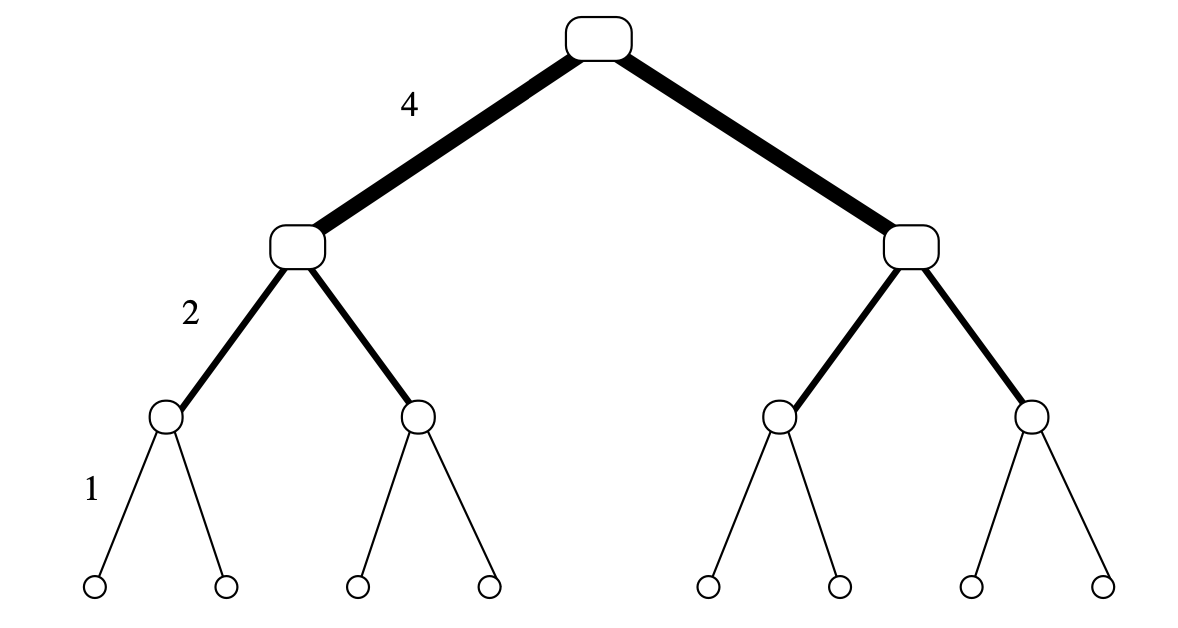
\includegraphics[width=\linewidth]{fat_tree.png}
\end{center}

Another topology are tori and meshes: Let $m,d \in \N$, the $(m,d)$-mesh $M$ is a graph with node set $V = [m]^d$ (vectors of length $d$ of numbers $\{1,...,n\}$) and edge set
$$E = \left \{   \{(a_1,...,a_d), (b_1,...,b_d) \; | \; a_i, b_i \in [m], \sum_{i=1}^d |a_i, b_i| = 1 \} \right \}$$

The $(m,d)$-torus $T(m,d)$ is a graph that consists of an $(m,d)$-mesh and additionally wrap-around edges from nodes $(a_1, ..., a_{i-1}, m - 1, a_{i+1}, ..., a_d) $ to nodes $(a_1, ..., a_{i-1}, 0, a_{i+1}, ..., a_d)$ for all $i \in \{1, ...,d\}$ and all $a_j \in [m]$ with $j \neq i$. $M(m,1)$ is a path, $T(m,1)$ a cycle and $M(2,d) = T(2,d)$ a $d$-dimensional hypercube.

\begin{center}
	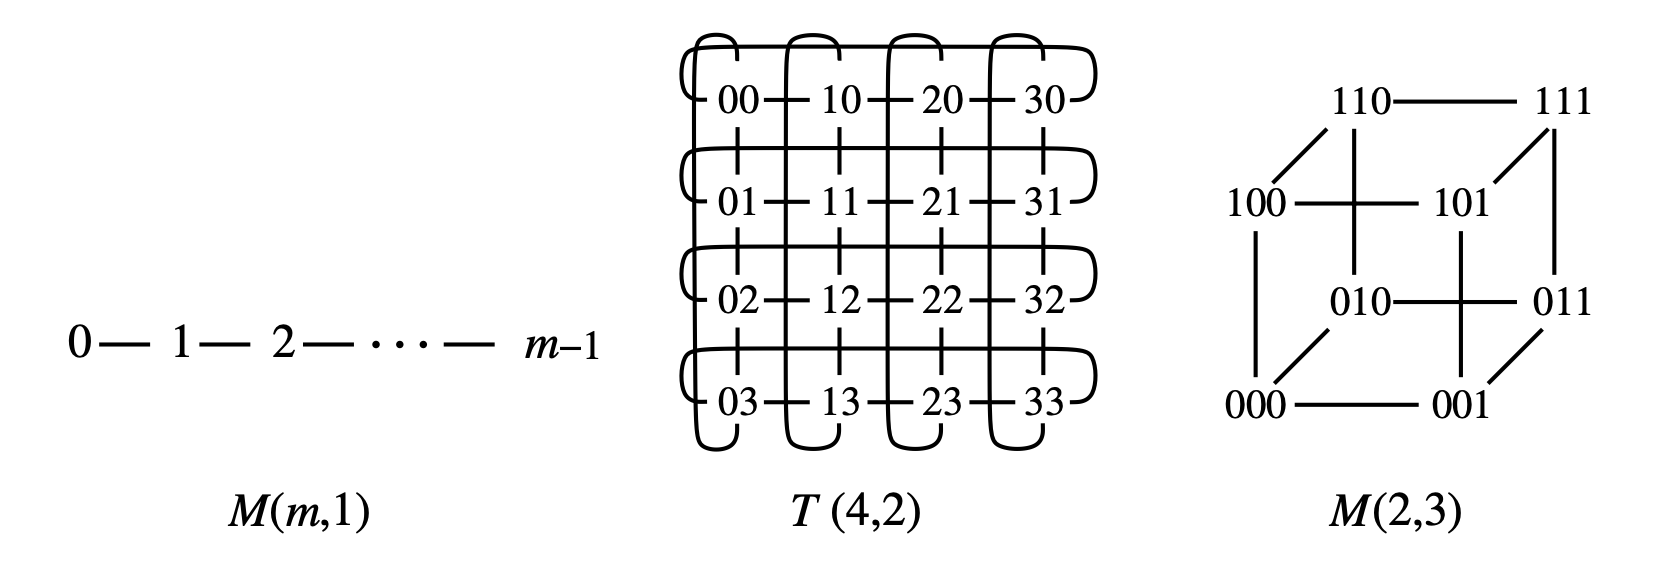
\includegraphics[width=\linewidth]{mesh.png}
\end{center}

Routing on a mesh, torus, or hypercube is trivial. On a $d$-dimensional hypercube, to get from a source bitstring $s$ to a target bitstring $t$ one only needs to fix each "wrong" bit, one at a time. There are $k!$ routes with $k$ hops. \medskip

We need to map the $d$-bit IDs to the universe $[0, 1)$. We can do so, by interpreting the bitstring $b = b_1 ... b_d$ as the number $\sum_{i=1}^d 2^{-i} b_i = (0.b_1 ... b_d)_2$ in binary. \medskip

There are many topologies that are similar to hypercubes, e.g. the Chord architecture. The hypercube connects every node with an ID in $[0,1)$ with every node in exactly distance $2^{-i}$. Chord instead connects nodes with approximately distance $2^{-i}$. Many of the following examples are also derivatives of hypercubes.

\subsubsection{Butterfly}

The $d$-dimensional butterfly $BF(d)$ is a graph with node set $V = [d+1] \times [2]^d$ and edge set $E = E_1 \cup E_2$ where:
$$E_1 = \{\{ (i, \alpha), (i+1, \alpha)\} \; | \; i \in [d], \alpha \in [2]^d\}$$
$$E_2 = \{\{ (i, \alpha), (i+1, \beta)\} \; | \; i \in [d], \alpha, \beta \in [2]^d, \alpha \oplus \beta = 2^i \}$$

The node set $\{(i, \alpha) \; | \; \alpha \in [2]^d\}$ forms the level $i$ of the butterfly. 
\begin{center}
	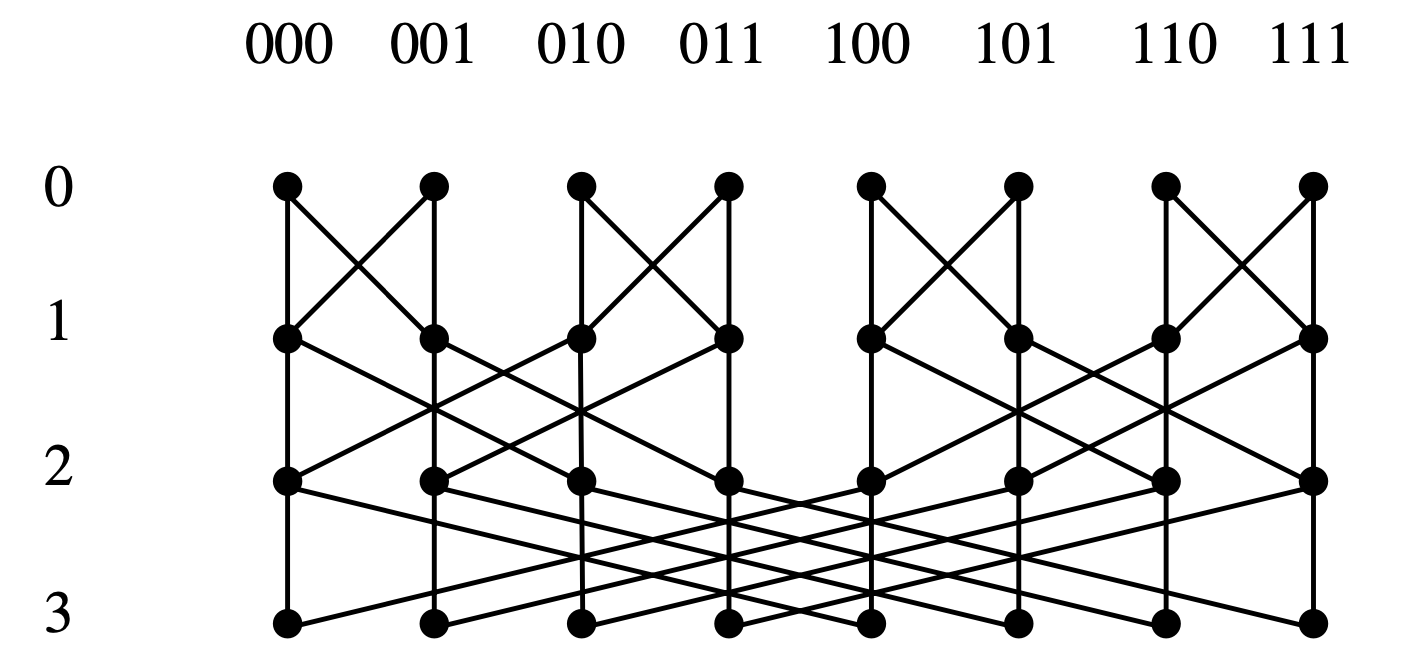
\includegraphics[width=0.8\linewidth]{butterfly.png}
\end{center}

The $d$-dimensional wrap-around butterfly $W - BF(d)$ is defined by taking the $BF(d)$ and having $(d, \alpha) = (0, \alpha)$ for all $\alpha$. \medskip

Butterflies have the advantage of a constant node degree over hypercubes, whereas hypercubes feature more fault-tolerant routing.

\subsubsection{Cube-Connected-Cycles}

The cube-connected-cycles network $CCC(d)$ is a graph with node set $V = \{ (a,p) \; | \; a \in [2]^d, p \in [d] \} $ and edge set \smallskip

$E = \{\{ (a,p), (a, p+1 \mod d) \} \; | \; \alpha \in [2]^d, p \in [d]\} \cup \{\{(a,p), (b,p)\} \; | \; a,b \in [2]^d, p \in [d], |a-b| = 2^p \}$ \smallskip

$CCC(3)$ results from the hypercube by replacing the corners by cycles. We can represent it in 2 different ways:
\begin{center}
	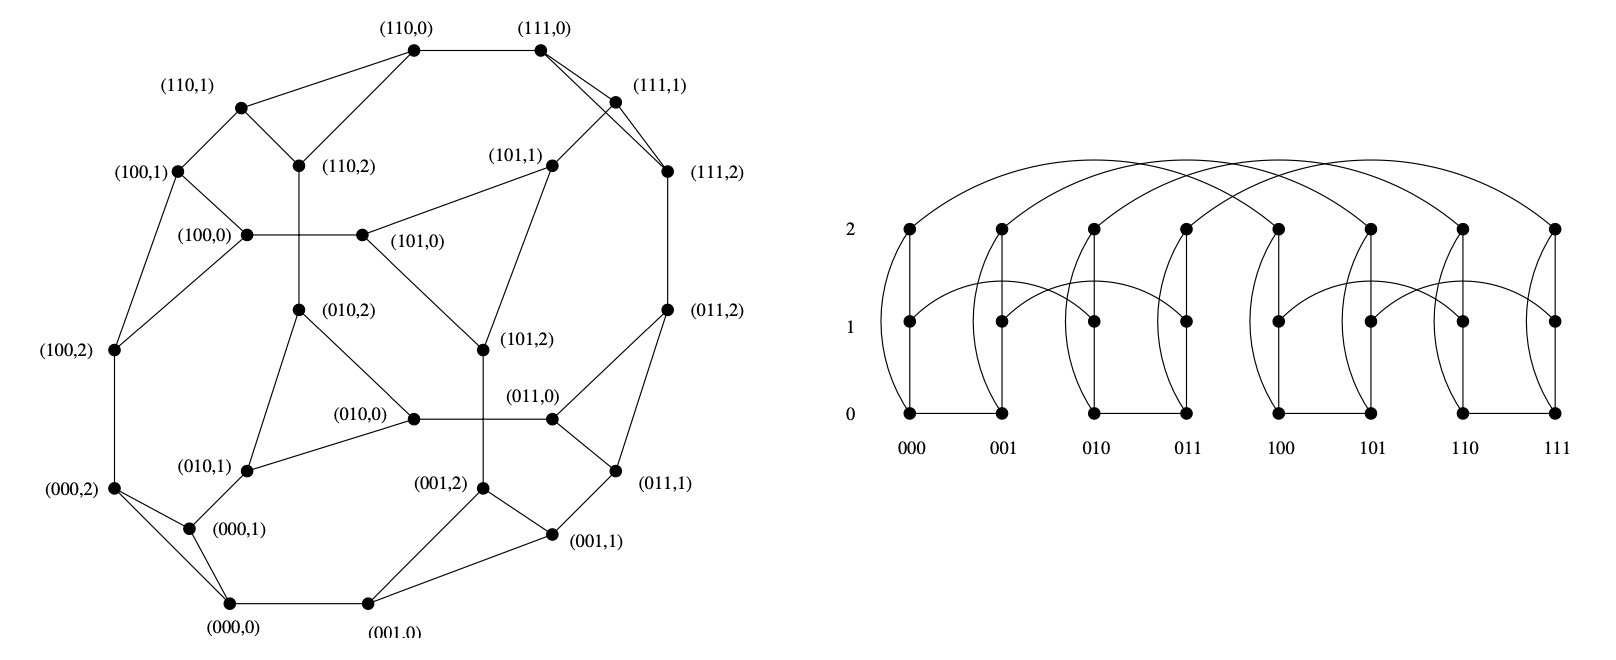
\includegraphics[width=\linewidth]{ccc.png}
\end{center}

\subsubsection{Shuffle-Exchange and DeBrujin}

The shuffle-exchange and the DeBruijn network are other ways of transforming the hypercubic interconnection structure into a constant degree network. \medskip

\textbf{Shuffle-Exchange}
\begin{center}
	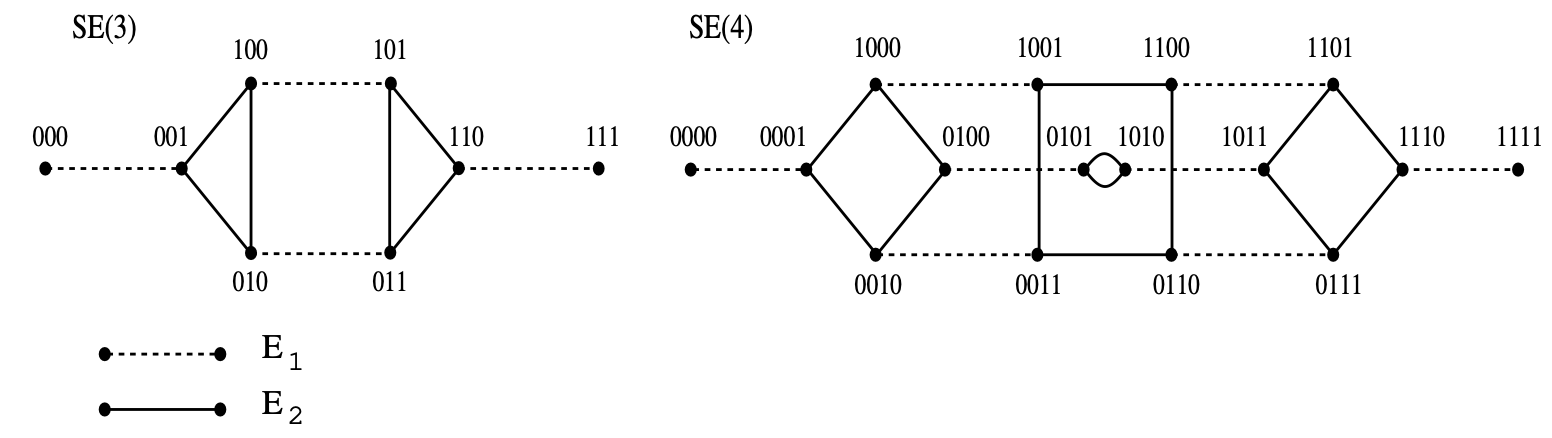
\includegraphics[width=0.9\linewidth]{shuffel_network.png}
\end{center}

\textbf{DeBrujin}
\begin{center}
	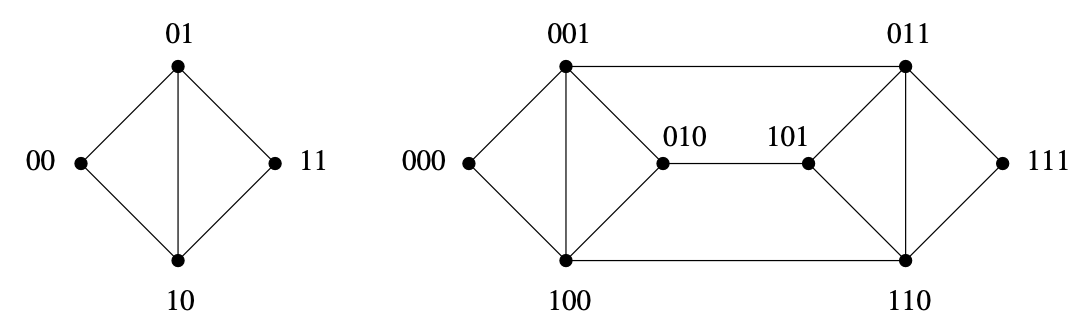
\includegraphics[width=0.9\linewidth]{debruijn.png}
\end{center}

\subsubsection{Skip List}

The skip list is an ordinary ordered linked list of objects, augmented with additional forward links. The ordinary linked list is the level 0 of the skip list. In addition, every object is promoted to level 1 with probability 1/2. As for level 0, all level 1 objects are connected by a linked list. In general, every object on level $i$ is promoted to the next level with probability 1/2. A special start-object points to the smallest/first object on each level. \medskip

Search, insert, and delete can be implemented in $\mathcal{O}(\log n)$ expected time in a skip list. There are obvious variants of the skip list, e.g., the skip graph. \medskip

Back to more general properties of hypercubic networks. In general, there is a trade o↵ between degree and diameter. Every graph of maximum degree $d > 2$ and size $n$ must have a diameter of at least $\lceil \log n / \log (d-1) \rceil -2$. In other words, constant-degree hypercubic networks feature an asymptotically optimal diameter $D$. Other hypercubic graphs manage to have a different tradeoff between node degree $d$ and diameter $D$.


\subsection{DHT and Churn}

A distributed hash table (DHT) is a distributed data structure that implements a distributed storage. A DHT should support at least (i) a search (for a key) and (ii) an insert (key, object) operation, possibly also (iii) a delete (key) operation. \medskip

A DHT can be implemented as a hypercubic overlay network with nodes having identifiers such that they span the ID space $[0, 1)$. We assume that a joining node knows a node which already belongs to the system. One way to do this is using some authority for a list of IP addresses of nodes that might be in the system. \medskip

To analyze this network against adversary, we assume that an adversary can remove and add a bounded number of nodes. It can choose which nodes to crash/join. Also, the adversary does not have to wait until the system is recovered before it crashes the next bash of nodes. \medskip

Our system is never fully repaired, but always fully functional. An adversary can add/remove at most $\mathcal O (\log n)$ nodes in a constant time interval. This covers repeatedly taking nodes down in a DDoS attack. Also we assume no message delays which can be achieved using time synchronization.\medskip

\begin{algorithm}[H]
\caption{DHT}
	Given: a globally known set of hash functions $h_i$ and a hypercube network \\
	Each hypercube virtual node ("hypernode") consist of $\Theta(\log n)$ nodes \\
	Nodes have connections to all other nodes of their hypernode and to nodes of their neighboring hypernodes \\
	Because of churn, some of the nodes have to change to another hypernode such that up to constant factors, all hypernodes own the same number of nodes at all times \\
	If the total number of nodes $n$ grows or shrinks above or below a certain threshold, the dimension of the hypercube is increased or decreased by one, respectively
\end{algorithm}
\medskip

Thus, each node has $\Theta(\log^2 n)$ neighbors. One can achieve $\Theta (\log n)$ with some additional effort. \medskip

The balancing of nodes can be seen as a dynamic token distribution problem on the hypercube. Each hypernode has a certain number of tokens and the goal is to distribute them along the edges s.t. all hypernodes end up with roughly the same number of tokens. \medskip

Using DHT with churn, we have a fully scalable, efficient distributed storage system which tolerates $\mathcal O(\log n)$ worse case joins and/or crashes per constant time interval. Nodes have $\mathcal O (\log n)$ overlay neighbors and search/insert take time $\mathcal O (\log n)$.



\section{Eventual Consistency}
\section{Advanced Blockchain}

\subsection{Selfish Mining}

A \textbf{selfish miner} hopes to earn the reward of a larger share of blocks than its hardware would allow. The selfish miner achieves this by temporarily keeping newly found blocks secret. \medskip

\begin{algorithm}[H]
\caption{Selfish Mining}
	Idea: Mine secretly, without immediately publishing newly found blocks\\
	Let $d_p$ be the depth of the public blockchain \\
	Let $d_s$ be the depth of the secretly mined blockchain\\
	\If{a new block $b_p$ is published}{
		\If{$d_s < d_p$}{
			Start mining on the newly found block $b_p$\\
		}
		\If{$d_p = d_s$}{
			Publish secretly mined block $b_s$\\
			Mine on $b_s$ and publish newly found block immediately
		}
		\If{$d_p = d_s - 1$}{
			Publish all secretly mined blocks
		}
	}
\end{algorithm}
\medskip

It may be rational to mine selfishly, depending on two parameters $\alpha$ and $\gamma$, where $\alpha$ is the ratio of the mining power of the selfishly miner, and $\gamma$ is the share of the altruistic mining power the selfishly miner can reach in the network if the selfishly miner publishes a block right after seeing a newly published block. Precisely, the selfishly miner share is:
$$\frac{\alpha(1-\alpha)^2(4\alpha + \gamma(1-2\alpha))-\alpha^3}{1 - (1 + (2- \alpha) \alpha)}$$

If the miner is honest (altruistic), then a miner with computational share $\alpha$ should expect to find an $\alpha$ fraction of the blocks.


\subsection{Ethereum}

\textbf{Ethereum} is a distributed state machine. Unlike Bitcoin, Ethereum promises to run arbitrary computer programs in a blockchain. \medskip

Like the Bitcoin network, Ethereum consists of nodes that are connected by a random virtual network. These nodes can join or leave the network arbitrarily. There is no central coordinator. Users broadcast cryptographically signed transactions in the network. Nodes collate these transactions and decide on the ordering of transactions by putting them in a block on the Ethereum blockchain. \medskip

\textbf{Smart contracts} are programs deployed on the Ethereum blockchain that have associated storage and can execute arbitrarily complex logic. They are written in higher level programming languages like Solidity, Vyper, etc. and are compiled down to EVM (Ethereum Virtual Machine) bytecode. They cannot be changed after deployment. But most smart contracts contain mutable storage, and this storage can be used to adapt the behavior of the smart contract. \medskip

Ethereum knows two kinds of accounts. \textbf{Externally Owned Accounts (EOAs)} are controlled by individuals, with a secret key. \textbf{Contract Accounts (CAs)} are for smart contracts. CAs are not controlled by a user. \medskip

An Ethereum \textbf{transaction} is sent by a user who controls an EOA to the Ethereum network. A transaction contains:
\begin{itemize}
	\item Nonce: This "number only used once" is simply a counter that counts how many transactions the account of the sender of the transaction has already sent.
	\item 160-bit address of the recipient.
	\item The transaction is signed by the user controlling the EOA.
	\item Value: The amount of Wei (the native currency of Ethereum) to transfer.
	\item Data: Optional data eld, which can be accessed by smart contracts.
	\item StartGas: A value representing the maximum amount of computation this transaction is allowed to use.
	\item GasPrice: How many Wei per unit of Gas the sender is paying. Miners will probably select transactions with a higher GasPrice.
\end{itemize}

There are three types of transactions:
\begin{itemize}
	\item A \textbf{Simple Transaction} in Ethereum transfers some of the native currency, called Wei, from one EOA to another.
	\item A \textbf{Smart Contract Creation Transaction} whose recipient address field is set to 0 and whose data field is set to compiled EVM code is used to deploy that code as a smart contract on the Ethereum blockchain. The contract is considered deployed after it has been mined in a block and is included in the blockchain at a sufficient depth.
	\item A \textbf{Smart Contract Execution Transaction} that has a smart contract address in its recipient field and code to execute a speciffic function of that contract in its data field.
\end{itemize}

Smart Contracts can execute computations, store data, send Ether to other accounts or smart contracts, and invoke other smart contracts. They can also be programmed to self destruct. This is the only way to remove them again from the Ethereum blockchain. Each contract stores data in 3 separate entities: storage, memory, and stack. Of these, only the storage area is persistent between transactions. \medskip

\textbf{Gas} is the unit of an atomic computation, like swapping two variables. Complex operations use more than 1 Gas, e.g., adding two numbers costs 3 Gas. \medskip

Transactions are an all or nothing affair. If the entire transaction could not be finished within the StartGas limit, an Out-of-Gas exception is raised. The state of the blockchain is reverted back to its values before the transaction. The amount of gas consumed is not returned back to the sender. \medskip

In Ethereum, like in Bitcoin, a \textbf{block} is a collection of transactions that is considered a part of the canonical history of transactions. Among other things, a block contains: pointers to parent and up to two uncles, the hash of the root node of a trie structure populated with each transaction of the block, the hash of the root node of the state trie (after transactions have been executed).

\section{Game Theory}

In this chapter, nodes no longer have a common goal but are selfish. They are not byzantine but try to benefit from a distributed system. Game theory attempts to mathematically capture behavior in strategic situations, in which an individual's success depends on the choices of others.

\subsection{Prisoner's Dilemma}

The following is one of the classical examples of game theory. Two prisoners $u, v$ are questioned by the police. They are both held in solitary confinement and cannot talk to each other. The prosecutors offer a bargain to each prisoner: snitch on the other prisoner to reduce your prison sentence.
\begin{center}
	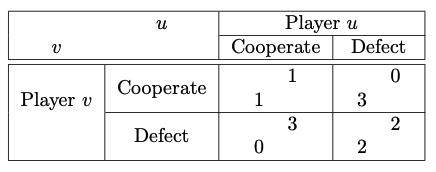
\includegraphics[width=0.8\linewidth]{prisoner.png}
\end{center}

A game requires at least two rational players, and each player can choose from at least two options (strategies). In every possible outcome (strategy profile) each player gets a certain payoff (or cost). The payoff of a player depends on the strategies of the other players. \medskip

A strategy profile is called \textbf{social optimum} (SO) if and only if it minimizes the sum of all costs (or maximizes payoff). \medskip

A strategy is \textbf{dominant} if a player is never worse off by playing this strategy. A dominant strategy profile is a strategy profile in which each player plays a dominant strategy. \medskip

A \textbf{Nash Equilibrium} (NE) is a strategy profile in which no player can improve by unilaterally (the strategies of the other players do not change) changing its strategy. A game can have multiple Nash Equilibria. If every player plays a dominant strategy, then this is by definition a Nash Equilibrium. \medskip

Nash Equilibria and dominant strategy profiles are so called solution concepts. They are used to analyze a game. \medskip

The \textbf{best response} is the best strategy given a belief about the strategy of the other players.


\subsection{Selfish Caching}

Consider computers in a network who want to access a file regularly. Each node $v \in V$ has a demand $d_v$ for the file and wants to minimize the cost for accessing it. To access it, a file can either be cached locally at cost 1 or be requested from another node $u$ with cost $c_{u \to v}$. If we interpret this game as a graph, then the cost $c_{u \to v}$ is equivalent to the length of the shortest path times the demand $d_v$.\medskip

\begin{algorithm}[H]
\caption{Nash Equilibrium for Selfish Mining}
	$S = \{\}$ \\
	\While{$V$ not empty}{
		Let $v$ be the node  maximum demand $d_v$ in $V$\\
		$S = S \cup \{v\}, \; V = V \backslash \{v\}$\\
		Remove every node $u$ from $V$ with $c_{v \to u} \leq 1$
	}
\end{algorithm}
\medskip

Let $NE_−$ denote the Nash Equilibrium with the highest cost (smallest payoff). The Price of Anarchy measures how much a distributed system degrades because of selfish nodes. The Price of Anarchy ($PoA$) is defined as:
$$PoA = \frac{\text{cost}(NE_-)}{\text{cost}(SO)}$$

Let $NE_+$ denote the Nash Equilibrium with the smallest cost (highest payoff). The Optimistic Price of Anarchy ($OPoA$) is defined as:
$$OPoA = \frac{\text{cost}(NE_+)}{\text{cost}(SO)}$$

We have $PoA \geq OPoA \geq 1$. The following shows a network with a Price of Anarchy of $\Theta (n)$

\begin{center}
	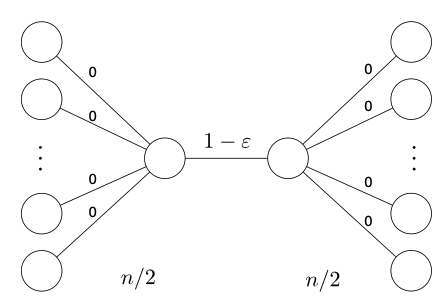
\includegraphics[width=0.7\linewidth]{selfish_caching.png}
\end{center}

The (Optimistic) Price of Anarchy of selfish caching can be $\Theta (n)$.


\subsection{Braess' Paradox}

Consider a game where cars want to travel from $s$ to $t$. Some road's cost depend on the amount of traffic going through them. There are 1000 cars. Adding a super fast road with delay 0 can increase the travel time from $s$ to $t$!
\begin{center}
	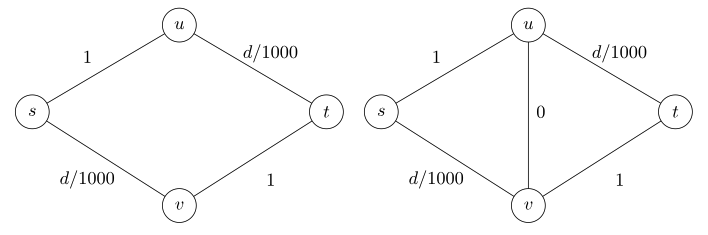
\includegraphics[width=\linewidth]{braess.png}
\end{center}

Each driver acts rationally, thus half of them takes the upper road and half of them the lower. The time for each traveler is then 1 + 500/1000 = 1.5. \medskip

If we introduce the new road with cost 0 between $u$ and $v$, each driver now drives from $s \to v \to u \to t$, leading to a total cost of $2 > 1.5$.


\subsection{Rock-Paper-Scissors}

We will consider the classical game of rock-paper-scissors. No strategy for one player is a Nash Equilibrium: whatever $u$ chooses, $v$ can always switch its strategy s.t. $v$ wins.
\begin{center}
	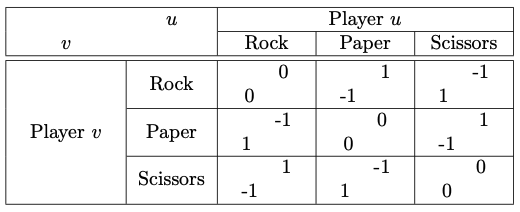
\includegraphics[width=\linewidth]{rps.png}
\end{center}

A \textbf{Mixed Nash Equilibrium} (MNE) is a strategy profile in which at least one player is playing a randomized strategy (choose strategy profiles according to probabilities), and no player can improve their expected payoff by unilaterally changing their (randomized) strategy. Every game has a mixed Nash Equilibrium.\medskip

The Nash Equilibrium of this game is if both players choose each strategy with probability 1/3.


\subsection{Mechanism Design}

Whereas game theory analyzes existing systems, there is a related area that focuses on designing games – mechanism design. The task is to create a game where nodes have an incentive to behave "nicely". \medskip

One good is sold to a group of bidders in an \textbf{auction}. Each bidder $v_i$ has a secret value $z_i$ for the good and tells his bid $b_i$ to the auctioneer. The auctioneer sells the good to one bidder for a price $p$. \medskip

For simplicity, we assume that no two bids are the same, and that $b_1 > b_2 > ...$\medskip

\begin{algorithm}[H]
\caption{First Price Auction}
	Every bidder $v_i$ submits his bid $b_i$\\
	The good is allocated to the highest bidder $v_1$ for the price $b_1 = p$
\end{algorithm}
\medskip

An auction is \textbf{truthful} if no player vi can gain anything by not stating the truth. A First Price Auction is not truthful. \medskip

\begin{algorithm}[H]
\caption{Second Price Auction}
	Every bidder $v_i$ submits his bid $b_i$\\
	The good is allocated to the highest bidder $v_1$ for the price $b_2 = p$
\end{algorithm}
\medskip

Truthful bidding is a dominant strategy in a Second Price Auction. \medskip

We can use this mechanism for selfish caching! We need one node who is first to cache. Every node says for which price it is willing to cache the file. We pay the node with the lowest offer and pay it the second lowest offer to ensure truthful offers. \medskip

Any Nash Equilibrium of Selfish Caching can be implemented for free. \medskip

Mechanism design assumes that the players act rationally and want to maximize their payoff. In real-world distributed systems some players may be not selfish, but actively malicious (byzantine).


\end{multicols*}
\end{document}

% ____ FOOTER ______________________________________________________
% Content and Template: 
% original by Danny Camenisch (dcamenisch@inf.ethz.ch), 2022
% based on different summaries from many helpful people